\documentclass{sigplanconf}
\usepackage{latexsym, mathrsfs}
\usepackage[usenames,dvipsnames]{color}
\usepackage[linesnumbered,ruled,procnumbered]{algorithm2e}
\usepackage{paralist}
\usepackage{xspace}
\usepackage{url}
\usepackage{graphicx}
\usepackage{floatflt}
\usepackage{times}
\usepackage{balance}
\usepackage{spverbatim}
\usepackage{hyperref}
\usepackage{amsmath}
\usepackage{subcaption} %{subfig}

\renewcommand*\ttdefault{cmvtt}
%\renewcommand*\familydefault{\ttdefault} %% Only if the base font of the document is to be typewriter style
\usepackage[T1]{fontenc}

\usepackage{cleveref}
\crefname{section}{\S\!\!\!\;}{\S\S}
\Crefname{section}{\S}{\S\S}

\usepackage[utf8]{inputenc} % make sure your Latex source has this, for accented chars

%COMPRESS
\newcommand{\squeezeup}{\vspace{-2.5mm}}
\DeclareMathOperator{\sign}{sign}


\usepackage{etoolbox}
\makeatletter
\patchcmd{\maketitle}{\@copyrightspace}{}{}{}
\makeatother

\newcommand{\q}[1]{{\vspace{.1in}\noindent \em {\bf Research Question}}}
\newenvironment{mydescription}{%
   \begin{description}{
           }
}{%
   \end{description}%
}
\newenvironment{denselist}{
    \begin{list}{\small{$\bullet$}}%
    {\setlength{\itemsep}{0ex} \setlength{\topsep}{0ex}
    \setlength{\parsep}{0pt} \setlength{\itemindent}{0pt}
    \setlength{\leftmargin}{1.5em}
    \setlength{\partopsep}{0pt}}}%
    {\end{list}}


\makeatletter
\def\@copyrightspace{\relax}
\makeatother


\newcommand{\topic}[1]{\vspace{1pt} \noindent \underline{\bf #1}}
%\theoremstyle{slplain}
\newtheorem{theorem}{Theorem}
\newtheorem{lemma}{Lemma}
\newtheorem{conjecture}{Conjecture}
\newtheorem{example}{Example}
\newtheorem{formulation}{Problem}
\newtheorem{definition}{Definition}
\newtheorem{observation}[theorem]{\textbf{Observation}}
\newtheorem{claim}[lemma]{\textbf{Claim}}
\newtheorem{problem}{\textbf{Problem}}
\newcommand{\stitle}[1]{\vspace{0.5em}\noindent\textbf{#1}}

\newcommand{\mm}{\small{\mathcal{M}}\xspace}
\newcommand{\ff}{\small{\mathcal{F}}\xspace}
\newcommand{\sss}{\small{\mathcal{S}}\xspace}

\newcommand{\topk}{{\sc Top-k}\xspace}
\newcommand{\genviz}{{\sc Genvisage}\xspace}
\newcommand{\earlyT}{{\sc EarlyTerm}\xspace}
\newcommand{\sampling}{{\sc Sampling}\xspace}
\newcommand{\traversal}{{\sc Traversal}\xspace}
%\newcommand{\ss}[1]{\noindent{\textcolor{red}{[Saurabh: #1]}}}
\newcommand{\agp}[1]{\noindent{\textcolor{RedOrange}{[Aditya: #1]}}}
\newcommand{\cb}[1]{\noindent{\textcolor{magenta}{[Charles: #1]}}}
\newcommand{\silu}[1]{\noindent{\textcolor{blue}{[Silu: #1]}}}

\newcommand{\expn}[1]{\noindent{\textcolor{blue}{[Expand?]: #1}}}
\newcommand{\cut}[1]{}
\newcommand{\todo}[1]{\noindent{\textcolor{red}{\textbf{[TODO]: #1}}}}
\newcommand{\trim}[1]{\noindent{\textcolor{magenta}{[Reduce?]: #1}}}

\newcommand{\eat}[1]{}

\newcommand{\papertext}[1]{\noindent{\textcolor{blue}{PAPER: #1}}}
%\newcommand{\tr}[1]{\noindent{\textcolor{red}{#1}}}
\newcommand{\tr}[1]{}
%\newcommand{\tleftout}[1]{\noindent{\textcolor{blue}{#1}}}
\newcommand{\tleftout}[1]{}

\newcommand{\squishlist}{\begin{list}{$\bullet$}{\leftmargin=1.2em \topsep 1pt \itemsep -1pt \parsep 1pt}}
\newcommand{\squishend}{\end{list}}
\newcommand{\sampar}[1]{\vspace{3pt}\noindent{\bf #1}}
\begin{document}
\title{\genviz: Rapid Identification of Visually Explainable Features for Genomic Data Analysis}


\authorinfo{xxx}
       {University of Illinois (UIUC)}
        {\url{xxx@illinois.edu}}


\maketitle

%!TEX root=separability.tex

%====================================================================
\section{Introduction}
\label{sec:intro}

A common approach to discovery in biology
is to construct experiments or analyses that directly
contrast two specific classes of biological objects.
Examples of this include examining patient samples
contrasting tumor versus normal tissue \needcite{},
studying the differences in molecular effects
of two competing drug treatments \needcite{},
or characterizing differentially expressed genes
compared to genes with unaltered gene expression
in a carefully designed experiment \needcite{}.
As is often the case with genomics, these
biological objects (e.g., tissue samples or drug experiments)
are frequently represented by high dimensional numeric feature vectors (e.g., tens of thousands of transcript abundance measurements).
To understand the mechanisms that lead to or
explain these two object classes,
researchers often employ statistical and
machine learning tools to identify a
manageable subset of features that
accentuate or explain the differences between them.
We term this the {\em separability problem}.
Often, researchers address this problem
by ranking each individual feature
using statistical tests \needcite{}
and univariate classifiers \needcite{}.
These approaches are fast
and scale linearly in the number of features,
but do not offer insight into the interplay
between important features that can provide a better
explanation or characterization of the factors or features
that separate the two object classes.
Alternatively, larger subsets of separating
features can be identified by more complex machine learning approaches, such as multivariate regression with LASSO regularization \needcite{} or pattern mining from random forest models \needcite{Han paper}.
However, running these machine learning methods on datasets with tens of thousands of features is extremely time-intensive.
Motivated by these observations,
we sought to build a tool that strikes a balance between the
two above-mentioned ``extreme''
strategies, enabling us to retrieve more than just the best {\em singular} features, and doing so in an {\em interactive} manner.

We present \genviz,
an interactive data exploration tool to address the separability problem.
Given a matrix of values for object features
and two labeled object sets, \genviz rapidly identifies
the top ranking pairs of features
that most clearly separate the objects of
the different classes.
We demonstrate that the feature pairs identified by \genviz more significantly
discriminate between the object classes than the corresponding
best ranking individual features.
Thus, by focusing on separating feature pairs, \genviz
offers researchers the ability to gain additional
insight beyond singular features, without the prolonged waiting time
needed to train a complex machine learning model.
Moreover, the identified feature pairs can be effortlessly
visualized in a two-dimensional interface.
However, quickly identifying top feature pairs
in typical biological datasets with many features
is a challenging task due to some fundamental limitations:
first, the number of feature pairs can be large;
second, the feature-object matrix must be examined
multiple times to evaluate the separability of
each feature pair;
and third, any precomputation to reduce latency
would be useless, given that
object sets may be provided on-the-fly.
For example, if objects corresponded to experimental
conditions, and features were gene expression measurements,
having about $20K$ gene features
means that we need to evaluate nearly $200M$ feature pairs,
and for each feature pair we need to at least scan all of the objects,
say $100K$ objects, if using a naive approach.
Therefore, sophisticated methods are required
to make the task of ranking feature pairs interactive.

\begin{figure*}[t]
 \centering
 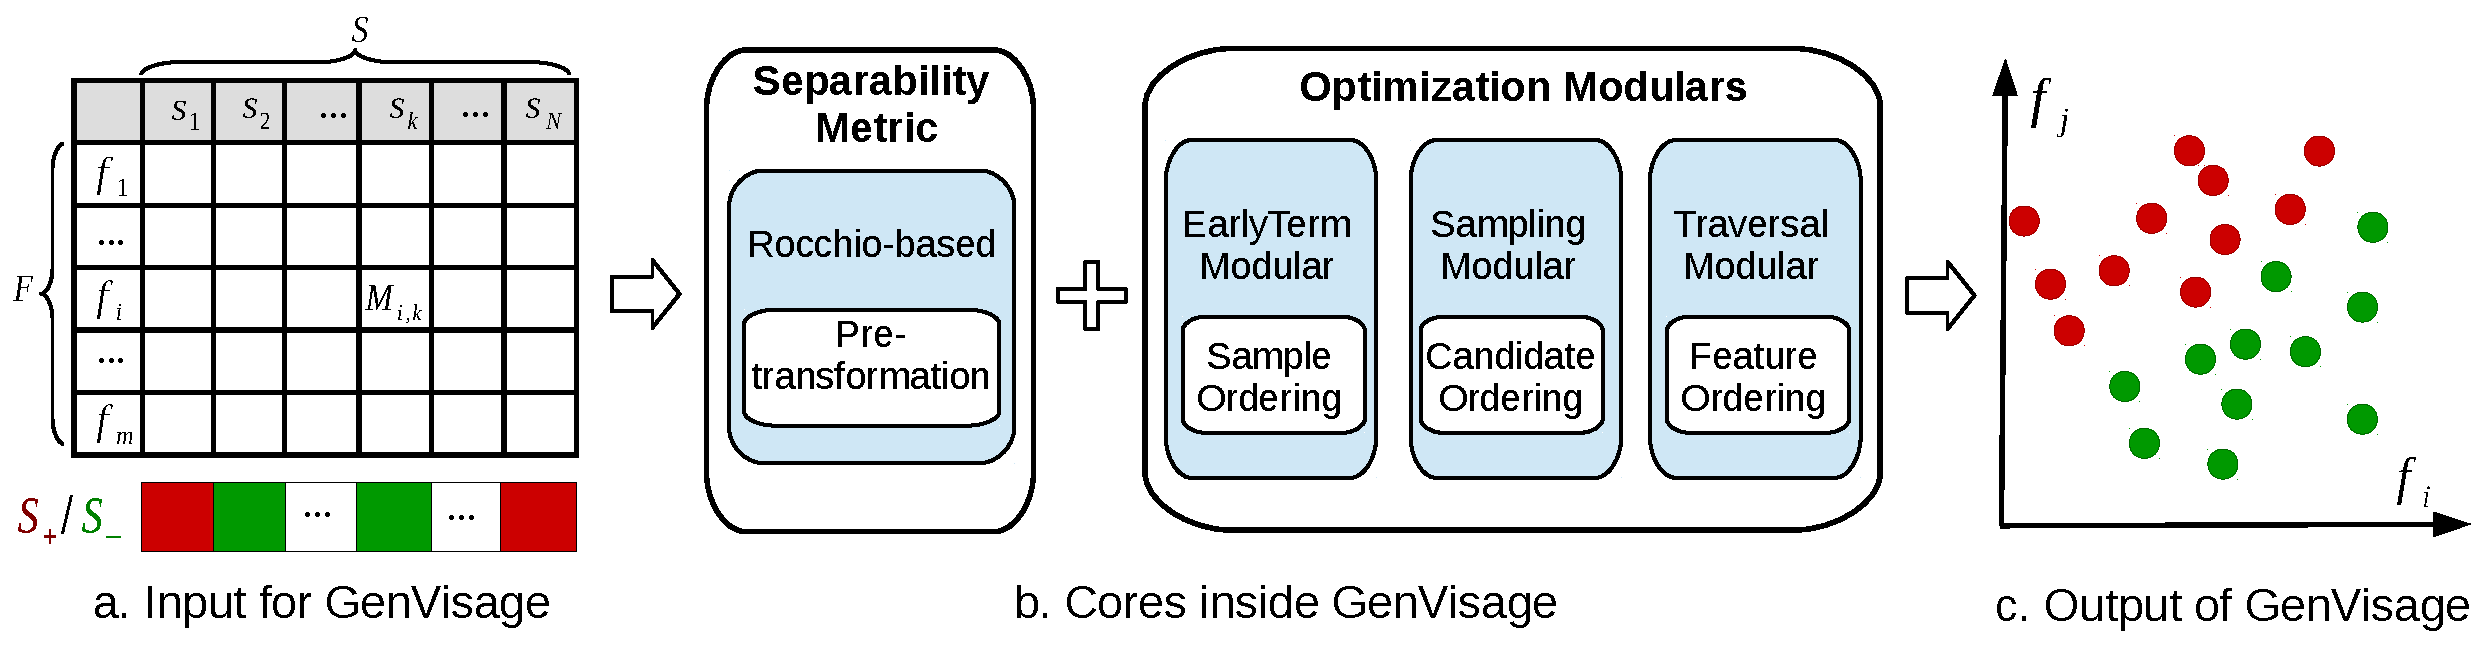
\includegraphics[width=0.9\linewidth]{fig/workflow2.pdf}
 \vspace{-10pt}
\caption{Overall \genviz Workflow.
Given (a) a feature-object matrix and positive and negative class labels on the objects, where red refers to the negative objects and green refers to the positive objects, \genviz (b) evaluates all pairs of features using several optimizations to identify (c) the top feature pair(s) and its corresponding visualization that best separates the object classes.}
\label{fig:workflow}
\vspace{-10pt}
\end{figure*}


In developing \genviz,
we identified a measure to score the separability
of a given feature pair for two object classes
that is conducive to
optimization techniques for enabling rapid
computation of feature pair rankings, while at
the same time providing an intuitive way to interpret
the resulting visualizations.
Satisfying both of these requirements enables \genviz to offer separability analysis in a responsive exploration environment that promotes the generation and prioritization of hypotheses for further investigation. Specifically, we develop various novel optimizations to make \genviz more interactive, targeting: {\em (a)} how to eliminate repeated computations; {\em (b)} how to prune feature pairs during early execution; {\em (c)} how to use sampling techniques to further reduce running time but with a statistical guarantee; and {\em (d)} how to traverse the search space of all feature pairs for improved efficiency.
While similar optimizations have been used in other settings,
e.g., sampling for approximate computation\needcite{},
the techniques need to be adapted for the separability problem.

We applied our \genviz tool to two genomic datasets.
In one, called \lincs, we find pairs of genes
whose expression discriminates between perturbagen experiments
of different drugs and in the other, called \msig,
we find pairs of annotations (such as pathway membership)
that separates differentially expressed cancer genes from all others.
Both of these applications are on objects with high-dimensional feature vectors,
so it is computationally expensive to score the separability
for all possible feature pairs.
With the \genviz tool, its carefully designed linear separability metric,
and its suite of sophisticated optimizations that alter how to and which feature pairs to evaluate,
we are able to {\bf \em accurately return the highest ranking separating
feature pairs for both datasets  within two minutes}.
This reflects a {\bf \em 180X} and {\bf \em 400X} speedup
over a competitive baseline for the \msig and \lincs data sets respectively.
With this speedup, \genviz enables researchers to quickly explore their data,
identify the strongest, most compelling features,
and form hypotheses about the interplay between them and with the object classes.
It also allows researchers to investigate different definitions
of the object classes on the fly, interactively,
and investigate alternative hypotheses,
as well as set up more in-depth,
longer machine learning based analysis that builds upon the \genviz results.

We further performed an in-depth analysis
for nine drugs in the \lincs dataset and
found 1070 feature pairs that more significantly
separated the perturbagen experiments than their
corresponding single features and were enriched
in literature support for known relationships between the genes and the drug,
as well as between the pair of genes themselves.

\genviz is available as a web-based tool at \url{knowcluster03.knoweng.org:9581}
\cb{change} and is open-sourced at \url{https://github.com/KnowEnG/Genvisage}.
\silu{add screenshot}


%==================================================================
\section{Methods}
\label{sec:method}
We begin by formally defining the {\em separability} problem,
introduce our separability metric,
and finally detail several optimizations that enable
the rapid identification of the best separating feature pairs.

%==================================================================
\subsection{Problem Definition}\label{sec:prob}

Let $\mm$ be a feature-object matrix of size $m\times N$, where each row is a feature and each column is an object as shown in Figure~\ref{fig:workflow}(a). An example feature-object matrix is one where each object corresponds to a tissue sample from a cancer patient and each feature correspond to a gene, such that the $(i,j)^{th}$ entry represents the expression level of the $i^{th}$ gene in the $j^{th}$ tissue sample. We denote the $m$ features as $\ff=\{f_1,f_2,\cdots,f_m\}$ and $N$ objects as $\oo=\{o_1,o_2,\cdots,o_N\}$. Each entry $\mm_{i,j}$ in $\mm$ corresponds
to the value of feature $f_i$ for object $o_j$ as illustrated in Figure~\ref{fig:workflow}(a).

In addition, we are given two non-overlapping sets of objects, one with a positive label and the other with a negative label, denoted as $\oo_+$ and $\oo_-$ respectively. Both sets are disjoint subsets of all objects, i.e., $\oo_+, \oo_-\subset \oo$, and $\oo_+\cap \oo_- = \emptyset$. In our example, we may have the tumor samples, $\oo_+$, be assigned the positive label, and the healthy tissue samples, $\oo_-$, be assigned the negative label. Let $\widehat{\oo}$ be the union of positive and negative objects and $n$ be the total number of labeled objects, i.e., $\widehat{\oo}=\oo_+\cup \oo_-$, $n=|\widehat{\oo}|$; $n\leq N$. Also, let $l_k$ be the label of object $o_k\in \widehat{\oo}$, i.e., $l_k=1$ if $o_k$ is positive and $l_k=-1$ if $o_k$ is negative.

The goal of \genviz is as follows: given a matrix $\mm$ and two object sets $\oo_+$ and $\oo_-$ as depicted in Figure~\ref{fig:workflow}(a), \genviz aims to find feature pairs that offer the best separation of objects in $\oo_+$ from those in $\oo_-$ represented by only those two features, and output a visualization that demonstrates the separability as shown in Figure~\ref{fig:workflow}(c). (We will define the metric for separability subsequently.) A feature pair that leads to a good ``visual'' separation between the positive and the negative sets may be able to explain or characterize the differences between the two via a interesting, complex relationship of the features. The overall workflow is depicted in Figure~\ref{fig:workflow}.
% Since we intend \genviz to be an interactive data exploration tool to be employed before more time-consuming machine learning methods, we allow for minor sacrifices to its accuracy in exchange for substantial improvements in its running time.
We formally define the separability problem as follows.
\begin{formulation}[Separability]\label{prob:separability}
Given a feature-object matrix $\mm$ and two labeled object sets $(\oo_+,\oo_-)$, rapidly identify the \topk feature pairs $(f_i,f_j)$ separating $\oo_+$ from $\oo_-$ based on a given separability metric, and produce their corresponding {visualizations}.
\end{formulation}
\noindent %Here a separability metric is a scoring function for any given feature pair, and \topk feature pairs refer to the $k$ feature pairs with the highest score under the separability metric.
We will describe our separability metric in Section~\ref{sec:metric}, and then discuss optimization techniques in Section~\ref{sec:opt}. Table~\ref{tbl:notation} summarizes our notation.



%==================================================================
\subsection{Separability Metric}\label{sec:metric}

Given a feature pair $(f_i,f_j)$ as axes, we can visualize the object sets $\oo_+$ and $\oo_-$ in a 2-D space, where each object corresponds to a point with x-value and y-value as the object's value on feature $f_i$ and $f_j$ respectively. A desirable (i.e., both interesting and interpretable) visualization would be one in which the objects are {\em linearly separated}, defined as follows. Two sets of objects, i.e., $\oo_+$ and $\oo_-$, are said to be \emph{linearly separable} if there exists at least one straight line in the 2-D space such that all points from $\oo_+$ are on one side of the line while all points from $\oo_-$ are on the other side.
We focus on metrics that capture this linear separation, since it corresponds to an intuitive 2-D visualization.
Given a feature pair $(f_i,f_j)$, we can represent a line $\ell$ as follows, where $x$ and $y$ represent an object's value on feature $f_i$ and $f_j$ respectively, and $w_0$, $w_i$ and $w_j$ are coefficients, where $w_j>0$.
\begin{equation}\label{eqn:line}
\begin{split}
\ell: \hspace{4mm} w_i\cdot x + w_j\cdot y +w_0 =0
\end{split}
\end{equation}
Given a feature pair $(f_i,f_j)$ and a line $\ell$, we can predict the label of an object $o_k$ based on the separating line in Equation~\ref{eqn:line}. Let $\eta_{i,j}^{\ell,k}$ be the predicted label of $o_k$, calculated using Equation~\ref{eqn:est_label} below:
\begin{equation}\label{eqn:est_label}
{\sf Predicted \hspace{1mm} Label:}\hspace{3mm} \eta_{i,j}^{\ell,k}=sign(w_i\cdot \mm_{i,k} + w_j\cdot \mm_{j,k} +w_0)
\end{equation}
\noindent If $o_k$ lies above the line $\ell$, i.e., $o_k$ has higher value on y-axis than the point on line $\ell$ with the same value on x-axis as $o_k$, then $\eta_{i,j}^{\ell,k}=1$; otherwise, $\eta_{i,j}^{\ell,k}=-1$. Let $\theta_{i,j}^{\ell,k}$ be the indicator variable denoting whether an object $o_k$ is correctly separated (i.e., the sign of the predicted label is the same as the real label $l_k$):
\begin{equation}\label{eqn:s_object}
\theta_{i,j}^{\ell,k}=\left\{
 \begin{array}{ll}
  1 \textit{\hspace{2mm} if \hspace{2mm}} \eta_{i,j}^{\ell,k}\cdot l_k = 1\\
  0 \textit{\hspace{2mm} otherwise \hspace{2mm}}
 \end{array}
 \right.
\end{equation}

\noindent If there is a line $\ell$ such that for every object $o_k\in \widehat{\oo}$, the object is correctly separated (i.e., $\theta_{i,j}^{\ell,k}$ = 1), then we say $\oo_+$ and $\oo_-$ are linearly separable.

% \begin{equation}\label{eqn:linear}
% \eta_{i,j}^{\ell,k} = \left\{
%  \begin{array}{ll}
%  1 \textit{\hspace{2mm} if \hspace{2mm}} o_k\in \oo_+, \textit{ i.e., } l_k=1 \\
%  -1 \textit{\hspace{2mm} if \hspace{2mm}} o_k\in \oo_-, \textit{ i.e., } l_k=-1
%  \end{array}
% \right.
% \end{equation}



For \genviz, we rank feature pairs by a separability metric based on {\em how well the objects in the feature pair's 2-D visualization can be linearly separated}, formally defined next.
%The basic intuition is that the users can easily recognize and interpret linear separability in a 2-D visualization. Thus if a visualization is perfectly linearly separated, it should have high score in our proposed separability metric; otherwise, we would find the best separating line $\ell$ in the visualization and report the largest number of correctly separated objects as the separability score.
Given a feature pair $(f_i, f_j)$ and a line $\ell$, the separability score of the line (denoted $\theta_{i, j}^\ell$) is defined as the sum of the indicators ($\theta_{i,j}^{\ell,k}$) for all objects, as shown in Equation~\ref{eqn:s_line}:
\begin{equation}\label{eqn:s_line}
\hspace{3mm} \theta_{i,j}^{\ell}= \sum_{k}{\theta_{i,j}^{\ell,k}}
\end{equation}
\noindent Figure~\ref{fig:brute_force} shows separability scores $\theta_{i, j}^\ell$ for different separating lines. For example, the separating line with $\theta_{i, j}^\ell=12$ correctly separates six green points and six red points. The final separability score for a feature pair $(f_i,f_j)$ (denoted as $\theta_{i, j}$) is defined as the best separability score $\theta_{i, j}^{\ell}$ among all possible lines $\ell$. Accordingly, we define the overall separability error of the feature pair as $err_{i,j}=n-\theta_{i, j}$.

%As shown in Equation~\ref{eqn:s_viz},
%\begin{equation}\label{eqn:s_viz}
%\hspace{3mm} \theta_{i,j}= \max_{\ell}\{\theta_{i,j}^{\ell}\} %{\sf Separability \hspace{1mm} %Score:}
%\end{equation}

%%%%%%%%%%%%%%%%%%%%%%%%%%%%%%%%%%NEED TOGGLE%%%%%%%%%%%%%%%%%%%%%%
% \begin{figure}[h]
% \centering
% \begin{subfigure}{0.235\textwidth}
% \centering
% 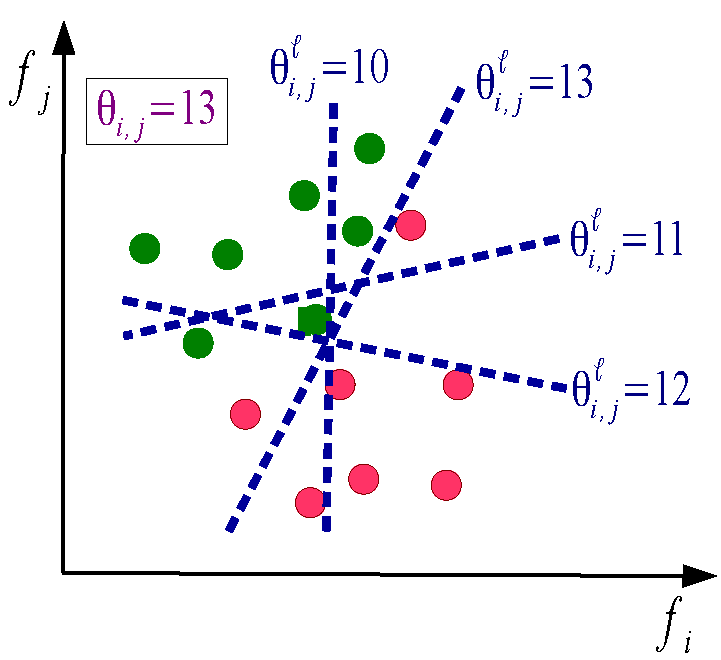
\includegraphics[width=\linewidth]{fig/metrics.pdf}
% \vspace{-5mm}
% \caption{Brute Force}%{$\theta_{i,j}^{\ell}$ with Different Lines[e]}
% \label{fig:brute_force}
% \end{subfigure}
% \begin{subfigure}{.235\textwidth}
% \centering
% 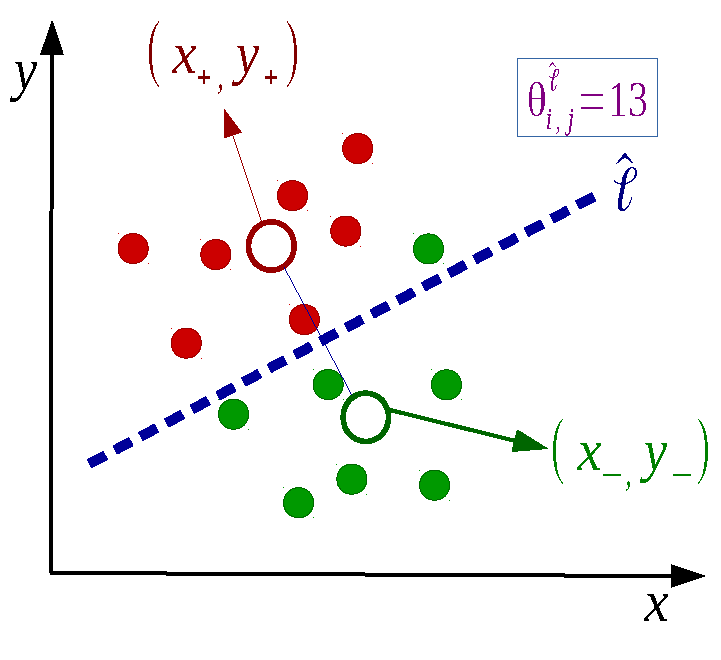
\includegraphics[width=\linewidth]{fig/rocchio.pdf}
% \vspace{-5mm}
% \caption{Rocchio-Based}%{$\theta_{i,j}^{\lhat}$ with Representative Line[f]}
% \label{fig:rocchio}
% \end{subfigure}
% \caption{Different methods to Calculate Separability Score $\theta_{i,j}$}
% \label{fig:metric}
% \end{figure}

\stitle{Brute Force Calculation of $\theta_{i,j}$.} As suggested in Figure~\ref{fig:brute_force}, the simplest way to calculate $\theta_{i,j}$ is to first enumerate all possible separating lines $\ell$ and calculate $\theta_{i,j}^\ell$ for each of them. This is infeasible as there are an infinite number of possible lines. However, we can easily trim down the search space to $O(n^2)$ lines by linking the points corresponding to every two objects in the 2-D plane. This is because the results of all other possible lines can be covered by these $O(n^2)$ lines~\cite{vapnik1998statistical}. Nevertheless, it is still very time-consuming to consider $O(n^2)$ lines for each feature pair $(f_i,f_j)$.

\begin{table}[t!]
\centering
\small
\begin{tabular}{|c|c|c|c|}
 \hline
 Symb. & Description & Symb. & Description\\
 \hline
 \hline
 $\mm$ & feature-object matrix & $\ff$ & feature set in $\mm$ \\
 \hline
 $f_i$ & feature $i$ in $\ff$ & $m$ & number of features in $\ff$\\
 \hline
 $\oo$ & object set in $\mm$ & $N$ & number of objects in $\oo$\\
 \hline
 $\oo_+$ & positive object set & $\oo_-$ & negative object set\\
 \hline
 $\widehat{\oo}$ & labelled object set & $n$ & number of labelled objects in $\widehat{\oo}$\\
 \hline
 $o_k$ & object $k$ in $\widehat{\oo}$ & $l_k$ & label of object $o_k$\\
 \hline
 $\ell$ & separating line in 2-D & $\lhat$ & representative line in 2-D\\
 \hline
 $\eta_{i,j}^{\ell,k}$ & predicted label of $o_k$ & $\theta_{i,j}^{\ell,k}$ & $o_k$ is correctly separated? \\
 \hline
 $\theta_{i,j}^{\ell}$ & \# correctly separated $o_k$ & $\theta_{i,j}$ & separability score\\
 \hline
 $\widehat{\mm}$ & $\mm$ after transformation & $\tilde{\theta}_{i,j}$ & estimated $\theta_{i,j}$\\
 \hline
 \end{tabular}
\caption{\genviz Method Notation}
\label{tbl:notation}
\vspace{-18pt}
\end{table}


\stitle{Rocchio-based Measure.} Rather than enumerating through the $O(n^2)$ possible lines to find the one with maximum $\theta_{i,j}^{\ell}$, we propose to speed up the process by intelligently selecting a single {\em representative line} $\lhat$ that will provide us with an estimated separability score, $\theta_{i,j}^{\lhat}$ that approximates the true linear separability score $\theta_{i, j}$.
%as shown in Equation~\ref{eqn:s_viz_appr}, .
%\begin{equation}\label{eqn:s_viz_appr}
%\theta_{i,j} \leftarrow \theta_{i,j}^{\lhat} %\approx
%\end{equation}
In order to achieve a fast and reliable estimate, we select our representative line based on Rocchio's algorithm~\cite{rocchio1971relevance}.
%As we will show later in Section~\ref{sec:exp}, $\theta_{i,j}^{\lhat}$ is comparable to $\theta_{i,j}$ when using Rocchio-based representative line $\lhat$. Let us describe in detail about the Rocchio-based representative line.
%The intuition behind using Rocchio's algorithm is that each object's predicted label should be the class label of its nearest class centroid.
More specifically, let us denote the centroids of positive objects $\oo_+$ and negative objects $\oo_-$ for a given $(f_i,f_j)$ as $\mu_{i,j}^+=(\mm_i^+,\mm_j^+)$ and $\mu_{i,j}^-=(\mm_i^-,\mm_j^-)$ respectively, where $\mm_i^+$ and $\mm_j^+$ are the values of the centroids of the positive objects on feature $f_i$ and $f_j$, and $\mm_i^-$ and $\mm_j^-$ are the values of the centroids of the negative objects on feature $f_i$ and $f_j$ respectively. The perpendicular bisector of the two centroids is selected as the representative separating line $\lhat$, following the template of Equation~\ref{eqn:line} with coefficients as in Equation~\ref{eqn:rep_line}:
%\lhat: \hspace{4mm} (\mm_i^+-\mm_i^-)\cdot x + (\mm_j^+-\mm_j^-)\cdot y -(\frac{(\mm_i^+)^2-(\mm_i^-)^2}{2}+\frac{(\mm_j^+)^2-(\mm_j^-)^2}{2}) =0
\begin{equation}\label{eqn:rep_line}
\begin{split}
& w_i = \mm_i^+-\mm_i^- \\
& w_j = \mm_j^+-\mm_j^- \\
& w_0 = -(\frac{(\mm_i^+)^2-(\mm_i^-)^2}{2}+\frac{(\mm_j^+)^2-(\mm_j^-)^2}{2})
\end{split}
\end{equation}
\noindent In Figure~\ref{fig:rocchio}, the "Rocchio-based" measure with the representative separating line $\theta_{i,j}^{\lhat}$ equals $13$ with one negative object (red point) mis-predicted as positive, while the true $\theta_{i,j}$ also equals $13$.

\stitle{Brute-force vs. Rocchio-based.} Compared to the brute force calculation, the Rocchio-based measure is much more light-weight in terms of running time, but at the cost of accuracy in calculating $\theta_{i,j}$. Intuitively, the representative line is a reasonable proxy to the best separating line since the Rocchio-based measure computes the centroids of the two classes as their representatives and assigns each object to its nearest centroid. We will further empirically demonstrate that $\theta_{i,j}^{\lhat}$ is a good proxy for $\theta_{i,j}$ in Section~\ref{sec:exp_comp}. Thus, we will focus on the Rocchio-based measure in the remainder of the manuscript, using $\theta_{i,j}$ and $\theta_{i,j}^{\lhat}$ interchangeably.
% \xagp{you have used Rocchio's alg/measure/representative line. Maybe avoid some of them for consistency.}


\begin{figure}[h]
\centering %%% not \center
\vspace{-5mm}
\subfigure[Brute Force]{\label{fig:brute_force}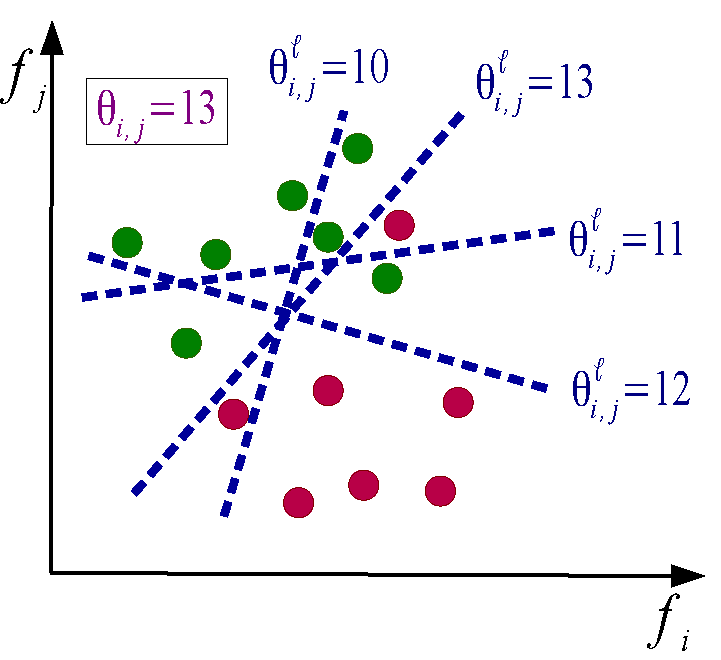
\includegraphics[width=.235\textwidth]{fig/metric.pdf}}
\subfigure[Rocchio-Based]{\label{fig:rocchio}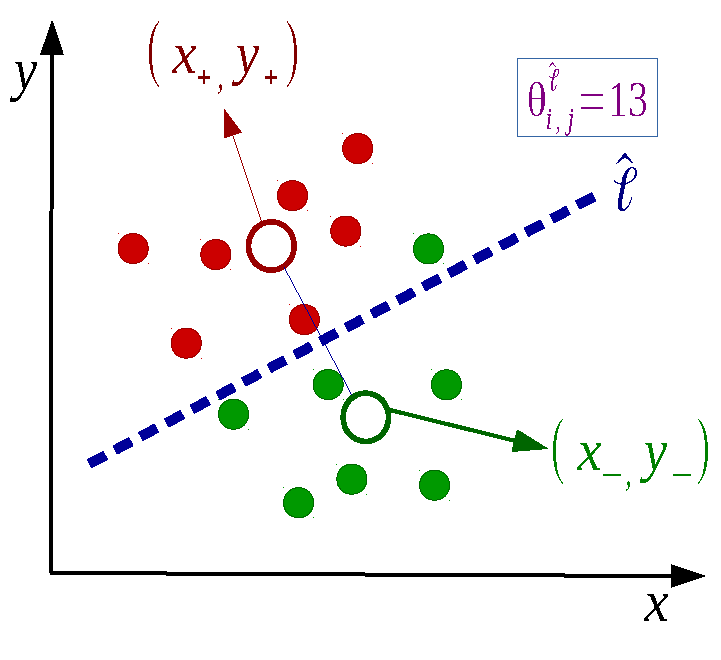
\includegraphics[width=.235\textwidth]{fig/rocchio.pdf}}
\vspace{-5mm}
\caption{Calculating Separability Score $\theta_{i,j}$. The scored separating line can be defined using (a) brute force or (b) the representative line from a Rocchio-based measure based on the object class centroids (white circles).}
\vspace{-5mm}
\label{fig:metric}
\end{figure}
%==================================================================
\subsection{Proposed Suite of Optimizations}\label{sec:opt}

In this section, we first analyze the time complexity of identifying the \topk feature pairs using the Rocchio-based measure, and then propose several optimization techniques to reduce the complexity.

\stitle{Time Complexity Analysis.} In order to calculate the separability of a given feature pair $(f_i, f_j)$, if we have already calculated the class centroids for each feature, the separating line $\lhat$ can be calculated in $O(1)$ time using Equation~\ref{eqn:rep_line}. We must then calculate the number of correctly separated objects $\theta_{i,j}^{\lhat}$ by evaluating all objects with respect to the line, i.e., $O(n)$ evaluations. Since there are $O(m^2)$ feature pair candidates, the total time complexity is $O(m^2n)$, which can be very large,
since $m$ and $n$ are typically large.

\stitle{Optimizations: Overview.} To reduce the time complexity, we introduce two categories of optimizations: First, those that reduce the amount of time required for fully evaluating a given feature pair and calculating its Rocchio-based measure (Section~\ref{ssec:trans},~\ref{ssec:earlyT}). Second, those that reduce the number of feature pairs that require full evaluation without dropping many feature pairs that are in the \topk (Section~\ref{ssec:sampling},~\ref{ssec:traversal}).

The first optimization module within the first category, \trans (Section~\ref{ssec:trans}), reduces redundant calculations across feature pairs by mapping the original feature-object matrix $\mm$ into a new space that enables faster evaluation of object labeling, and thus faster calculation of separability score. The second optimization module, \earlyT (Section~\ref{ssec:earlyT}), takes advantage of the fact that evaluation of a poorly separating feature pair can be terminated early without having to evaluate the separability of all $n$ objects.

The first optimization module within the second category, \sampling module (Section~\ref{ssec:sampling}) first identifies likely \topk feature pair candidates by evaluating their separability on a sampled subset of all objects, and then conducts full evaluations only on these feature pair candidates---thereby reducing the number of feature pairs that are fully evaluated. Finally, the \traversal module (Section~\ref{ssec:traversal}) reduces the number of feature pairs checked by greedily choosing feature pairs based on the separability of the corresponding single features. These optimization modules can be used on their own or combined with each other.

In Section~\ref{sec:exp}, we will show how these optimizations modules greatly reduce the running time of finding the \topk separating feature pairs without significantly affecting the accuracy.

%==================================================================
\subsubsection{Pre-Transformation for Faster Feature Pair Evaluation} \label{ssec:trans}

Let us review the process of computing the separability $\theta_{i,j}^{\lhat}$. Given a feature pair $(f_i,f_j)$ and the corresponding positive and negative centroids, {\em (i)} we first compute $w_0$, $w_i$ and $w_j$ for $\lhat$ based on Equation~\ref{eqn:rep_line}. Next, for each object $o_k$, {\em (ii)} we obtain the predicted label $\eta_{i,j}^{\lhat,k}$ according to Equation~\ref{eqn:est_label}. This step requires two multiplications and three additions. Finally, {\em (iii)} we calculate $\theta_{i,j}^{\lhat,k}$ and the separability $\theta_{i,j}^{\lhat}$ based on Equation~\ref{eqn:s_object} and \ref{eqn:s_line} respectively. This whole process is repeated for every feature pair candidate. However, there is massive redundancy across the processing of different feature pairs. For instance, when calculating the separability for two different feature pairs $(f_i,f_j)$ and $(f_i,f_{j'})$ with a common $f_i$, $w_i$ is in fact shared, and calculation of $w_i\cdot \mm_{i,k}$ in Equation~\ref{eqn:est_label} is repeated for each object $o_k$. Given this, we propose to first transform $\mm_{i,k}$ into another space to reduce this computational redundancy.
\sinha{is there another work we can cite that has done this?}

\stitle{High Level Idea.} The high level idea for \trans is to pre-calculate some common computational components across different feature pairs, and reuse these components when computing the separability for each feature pair, thereby eliminating repeated computation. In the following, we identify the common computations across different feature pairs, transform $\mm_{i,k}$ into another space using those components, and update the separability score equation accordingly.

\stitle{Details.} For each feature $f_i$, we find the average values of the positive and negative objects for that feature, $\mm_i^+$ and $\mm_i^-$ respectively, and then we pre-transform $\mm_{i,k}$, i.e., the value of object $o_k$ on the feature $i$, to $\widehat{\mm}_{i,k}$:
\begin{equation}\label{eqn:matrix_transform}
\widehat{\mm}_{i,k} = \Big( (\mm_i^+-\mm_i^-)\cdot \mm_{i,k}-\frac{(\mm_i^+)^2-(\mm_i^-)^2}{2} \Big) \cdot l_k
\end{equation}
\noindent The basic idea is to decompose Equation~\ref{eqn:est_label} into two components, with each one only related to a single, individual feature. This pre-transformation incorporates the class centroids into the matrix values, obviating their integration later for every feature pair that involves the given feature. Equation~\ref{eqn:matrix_transform} also multiplies in the class label of the object, $l_k$, rather than repeating this multiplication every time the object is evaluated. With this transformation of the feature-object matrix, evaluating whether an object was correctly separated is simplified from Equation~\ref{eqn:s_object} into Equation~\ref{eqn:s_object_transform}:
\agp{confusing because $L$ is not there in Equation~\ref{eqn:s_object}}\silu{maybe add "Since our focus is on Rocchio-based measure, we replace the separating line $\ell$ in Equation~\ref{eqn:s_object} with the representing line $L$ in Equation~\ref{eqn:s_object_transform}."}
%, and get rid of checking the real label $l_k$ in Equation~\ref{eqn:s_object}
\begin{equation}\label{eqn:s_object_transform}
\theta_{i,j}^{\lhat,k}=\left\{
 \begin{array}{ll}
  1 \textit{\hspace{2mm} if \hspace{2mm}} sign(\widehat{\mm}_{i,k} + \widehat{\mm}_{j,k}) = 1\\
  0 \textit{\hspace{2mm} otherwise \hspace{2mm}}
 \end{array}
 \right.
\end{equation}
%\begin{equation}\label{eqn:est_label_transform}
%\eta_{i,j}^{\lhat,k}=\sign(\widehat{\mm}_{i,k} + \widehat{\mm}_{j,k})
%\end{equation}
After pre-transformation, we are now ready to compute the separability score $\theta_{i,j}^{\lhat}$. Given a feature pair $(f_i,f_j)$, we can compute $\theta_{i,j}^{\lhat,k}$ for each object $o_k$ based on Equation~\ref{eqn:s_object_transform}. Note that this step only involves one addition and one comparison. Next, we can calculate overall separability score $\theta_{i,j}^{\lhat} = \sum_{k}{\theta_{i,j}^{\lhat,k}}$ similarly to Equation~\ref{eqn:s_line} without the pre-transformation. In all, compared to evaluations without the pre-transformation, we not only eliminate the steps of computing $w_0$, $w_i$ and $w_j$ for every feature pair, but also reduce the cost of calculating $\eta_{i,j}^{\lhat,k}$ in Equation~\ref{eqn:est_label}. In the following sections, we will consider $\widehat{\mm}$ instead of $\mm$, and Equation~\ref{eqn:s_object_transform} instead of Equation~\ref{eqn:est_label} and~\ref{eqn:s_object}.
%Hence, by conducting transformation in Equation~\ref{eqn:matrix_transform} and~\ref{eqn:s_object_transform}, we have mapped our problem to a new space.

\begin{figure}[h]
\centering %%% not \center
\vspace{-5mm}
\subfigure[Pre-Transformation]{\label{fig:transform}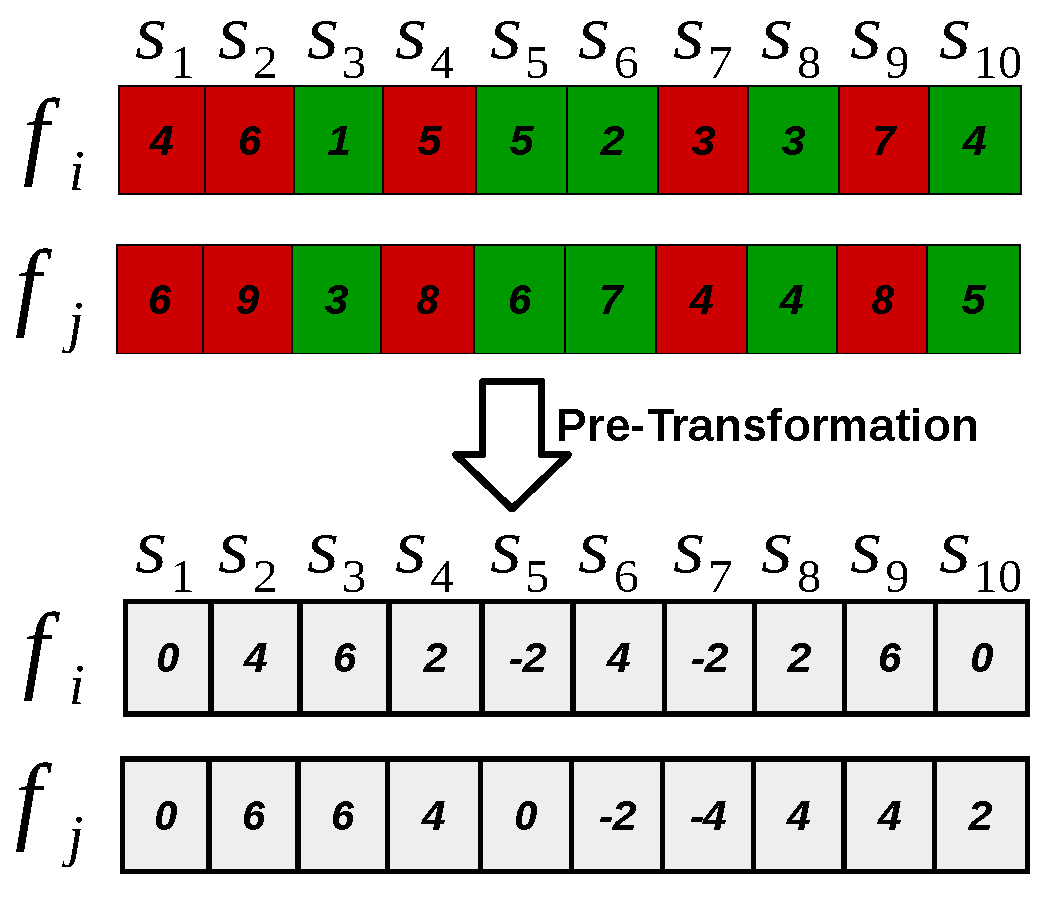
\includegraphics[width=.235\textwidth]{fig/transformation.pdf}}
\subfigure[Early Termination ($\tau = 1$)]{\label{fig:earlyT}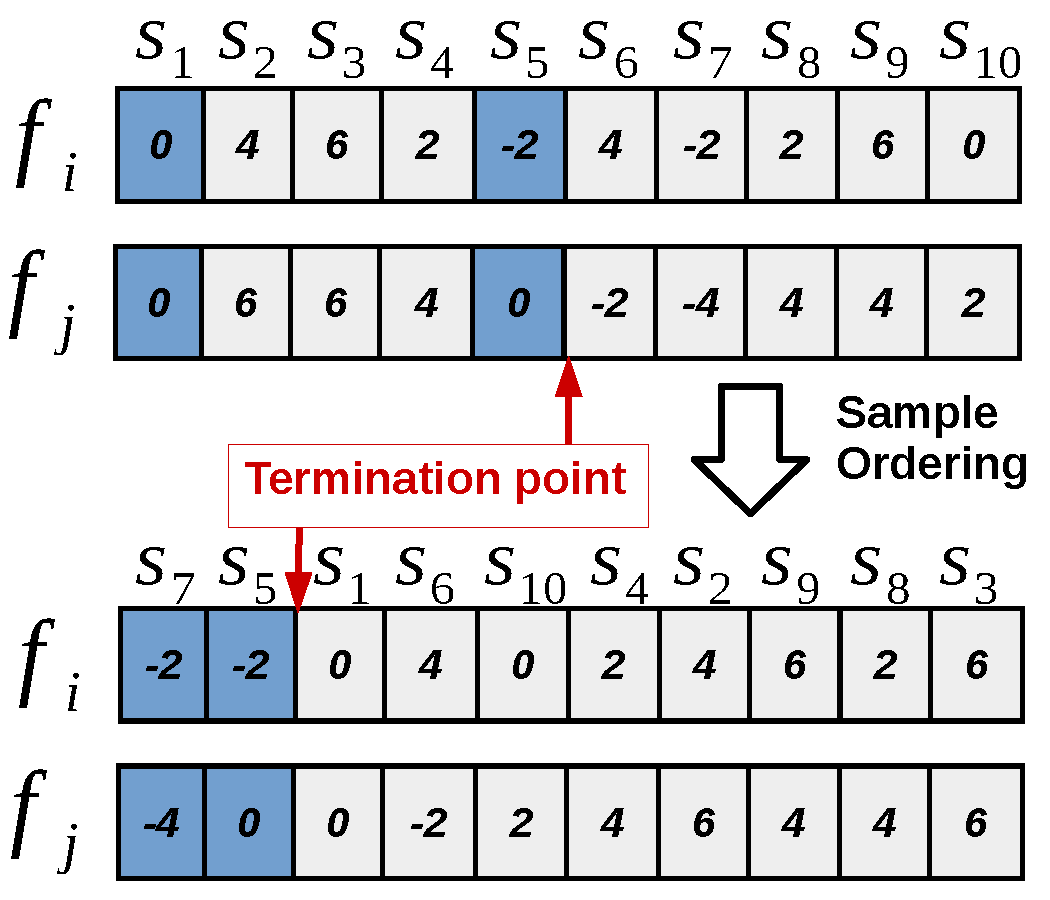
\includegraphics[width=.235\textwidth]{fig/earlyT.pdf}}
\vspace{-5mm}
\caption{Optimizations for Feature Pair Evaluation. (a) The \trans module is applied once to the original values in the feature-object matrix $\mm$ (above) using Equation~\ref{eqn:matrix_transform} to produce $\widehat{\mm}$ (below), which will reduce later calculations. (b) With the \earlyT module, a feature pair can be discarded from consideration for the \topk before all objects are evaluated (above) with even greater speedup potential after re-ordering the objects (below).}
\vspace{-8mm}
\label{fig:trans_term}
\end{figure}

\begin{example}[Transformation]
Figure~\ref{fig:transform} illustrates the transformation for two features, $f_i$ and $f_j$. The top half depicts $\mm_{i,k}$ and $\mm_{j,k}$ before transformation, where green color represents a positive label and red color represents a negative label. In this example, the centroids of the positive and negative objects are $\mu_{i,j}^+=(5,7)$ and $\mu_{i,j}^-=(3,5)$ respectively. Hence, we can rewrite Equation~\ref{eqn:matrix_transform} as $\widehat{\mm}_{i,k} = (2\mm_{i,k}-8)\cdot l_k$ and $\widehat{\mm}_{j,k} = (2\mm_{i,k}-12)\cdot l_k$ for features $f_i$ and $f_j$ respectively. After calculation, we can obtain the values for $\widehat{\mm}_{i,k}$ and $\widehat{\mm}_{j,k}$ shown in the bottom half of Figure~\ref{fig:transform}.
\end{example}

\sinha{at this point, write a summary of the time complexity of calculating $\theta_{i,j}^{\lhat}$ for a feature pair i,j using transformation (include preprocessing separately)}
\silu{the big-O time complexity is not changed. More precisely, only with constant improvement. Preprocessing takes O(mn) as we discussed in Results section.}
%%%%%%%%%%%%%%%%%%%%%%%%%%%%%%%%%%NEED TOGGLE%%%%%%%%%%%%%%%%%%%%%%
% \begin{figure}[h]
% \centering
% \begin{subfigure}{0.235\textwidth}
% \centering
% 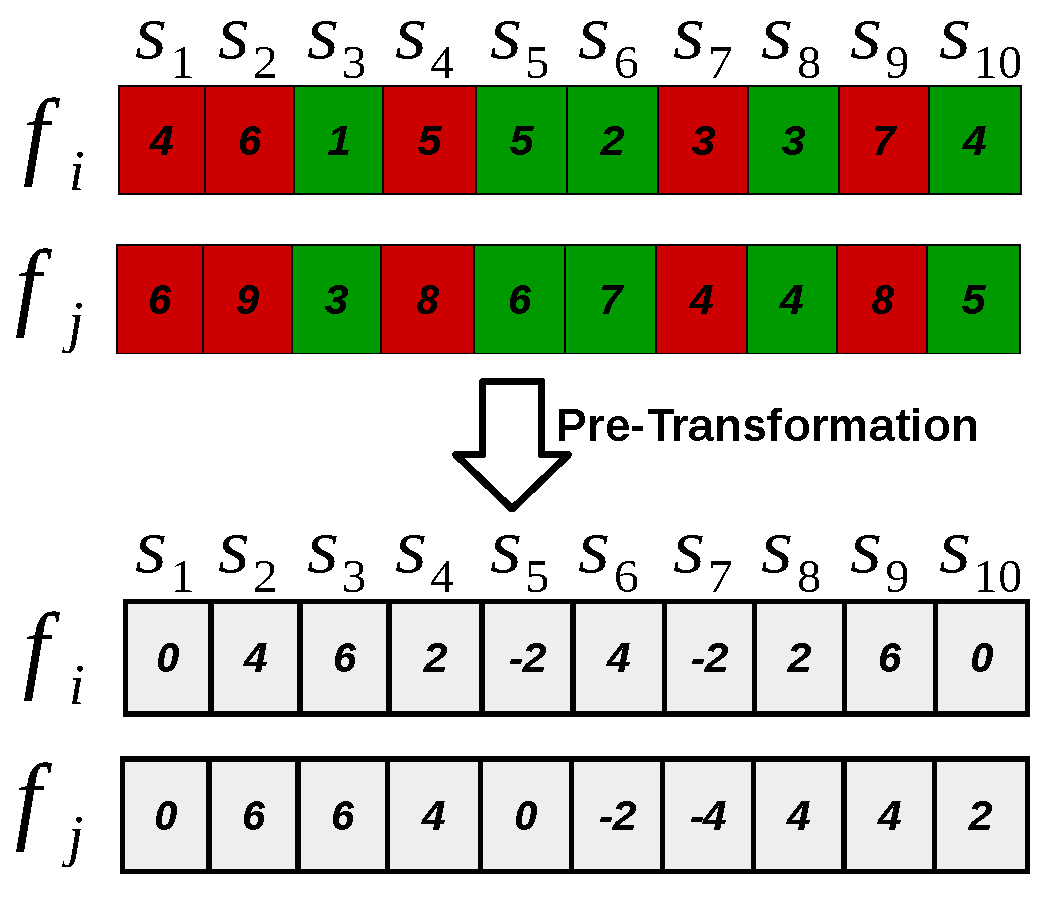
\includegraphics[width=\linewidth]{fig/transformation.pdf}
% \vspace{-5mm}
% \caption{Pre-Transformation}%{$\theta_{i,j}^{\ell}$ with Different Lines}
% \label{fig:transform}
% \end{subfigure}
% \begin{subfigure}{.235\textwidth}
% \centering
% 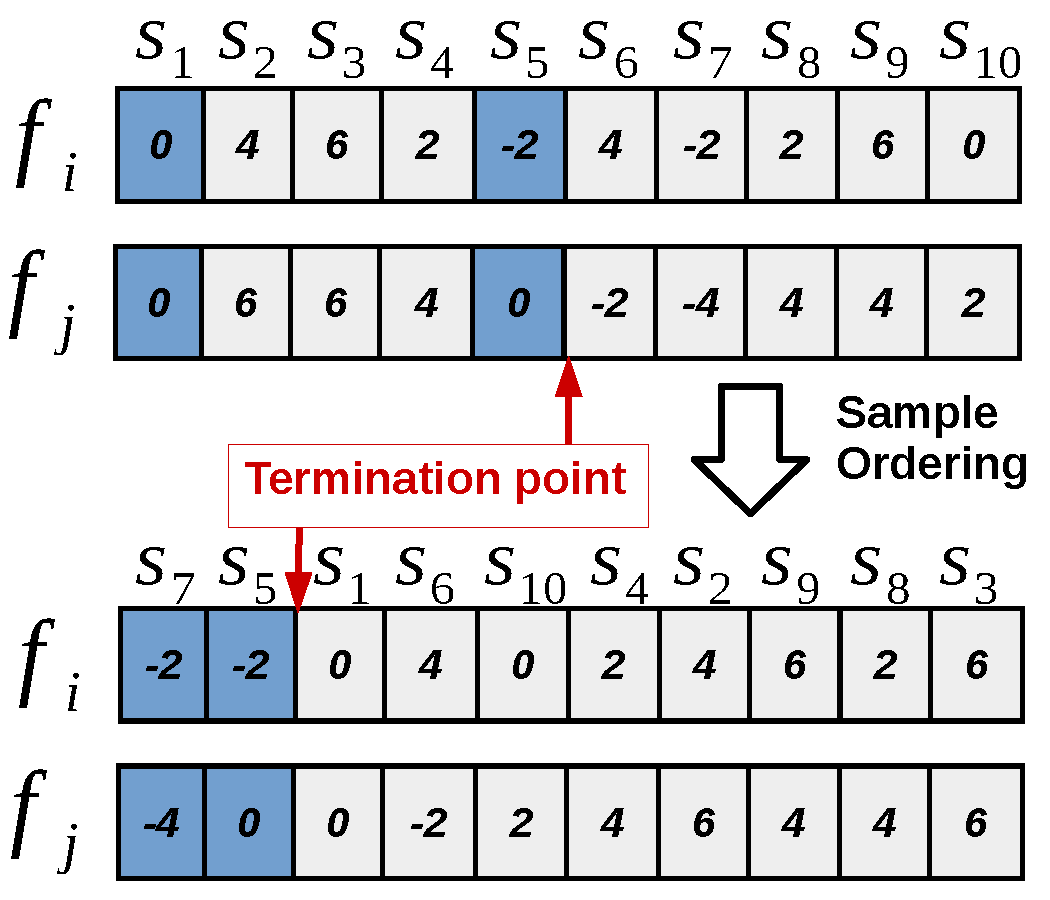
\includegraphics[width=\linewidth]{fig/earlyT.pdf}
% \vspace{-5mm}
% \caption{Early Termination ($\tau = 1$)}%{$\theta_{i,j}^{\lhat}$ with Representative Line}
% \label{fig:earlyT}
% \end{subfigure}
% \caption{Different Methods to Reduce Running Time}
% \label{fig:metric}
% \end{figure}

\agp{suggest delete next para; one line replacement: note that this approach can also be extended to the single feature case.} \silu{we can do that.}

\stitle{Extension to Single Features.} For a feature pair $(f_i,f_j)$ where $i=j$, we can treat the corresponding $\theta_{i,i}$ as the separability score for a single feature $f_i$. Equation~\ref{eqn:s_object_transform} can be further reduced to Equation~\ref{eqn:s_object_transform_single}.

\begin{equation}\label{eqn:s_object_transform_single}
\theta_{i,i}^{\lhat,k}=\left\{
 \begin{array}{ll}
  1 \textit{\hspace{2mm} if \hspace{2mm}} sign(\widehat{\mm}_{i,k}) = 1\\
  0 \textit{\hspace{2mm} otherwise \hspace{2mm}}
 \end{array}
 \right.
\end{equation}

Hence, we can calculate the separability score $\theta_{i,i}$ very efficiently for each single feature, based on the transformed matrix $\widehat{\mm}$.

%==================================================================
\subsubsection{Early Termination} \label{ssec:earlyT}

Given a feature pair $(f_i,f_j)$ and line $L$, we need to make a full scan of all objects to compute the separability score $\theta_{i,j}^{\lhat}$ according to Equation~\ref{eqn:s_line}. However, our goal is to not compute the separability score for all feature pairs, instead we only need to identify the \topk feature pairs. Thus, we propose to reduce the running time using early termination when scanning the objects, denoted as the \earlyT module as shown in Figure~\ref{fig:workflow}.

\stitle{High Level Idea.} The basic idea is to maintain a upper bound for the separability error $err_{i,j}$ of the \topk feature pairs, denoted as $\tau$. Correspondingly, the lower bound of the separability score can be denoted as ($n-\tau$), where $n$ is the total number of objects $\hat{\oo}$. Given a feature pair $(f_i,f_j)$, we start to scan the object list until the number of incorrectly classified objects exceeds $\tau$. If so, we can terminate early and prune this feature pair since it cannot be among the \topk feature pairs. Otherwise, if the number of incorrectly classified objects never exceeds $\tau$ during this scan, then $(f_i,f_j)$ is added to the \topk feature pair set and we update $\tau$ accordingly. Although \earlyT has the potential to always reduce the running time, its benefits are sensitive to the ordering of the objects for evaluation. Since we terminate as soon as we find $\tau$ incorrectly classified objects, we can improve our running time if we examine ``problematic'' objects that are unlikely to be correctly classified relatively early.

\stitle{Enhancement by Object Ordering.} To evaluate ``problematic'' objects earlier, we order the objects in descending order of the number of single features $f_i$ that incorrectly classify the object $o_k$, i.e., $\widehat{\mm}_{i,k}\leq0$. Thus, the first object evaluated is the one that is incorrectly classified by the most single features. We study the impact of this strategy in Section~\ref{sec:exp}.

\begin{example}[\earlyT \& Object Ordering]
Figure~\ref{fig:earlyT} illustrates how early termination and object ordering help reduce the running time. The top half depicts the $\widehat{\mm}$ after transformation. Say the current error upper bound is $\tau=1$. We start scanning the object list from left to right and determine whether each object is correctly separated based on Equation~\ref{eqn:s_object_transform}. Incorrectly classified objects are marked in blue, such as $o_1$, since $\widehat{\mm}_{i,1}+\widehat{\mm}_{j,1}\leq0$. We can terminate after evaluating $o_5$ since the number of incorrectly classified objects exceeds $\tau=1$.

The bottom half of Figure~\ref{fig:earlyT} shows $\widehat{\mm}$ after object reordering where "problematic" objects are placed on the left. In this way, after checking only the first two objects, we can terminate and eliminate this feature pair from further consideration.
\end{example}

\cb{note, 0's are treated as mis-labels and ties are broken randomly.}

%==================================================================
\subsubsection{Sampling-based Estimation} \label{ssec:sampling}

One downside of the \earlyT module, which reduces the number of examined objects, is that the improvement in the running time is highly data-dependent. Here, we propose a stochastic method, called \sampling, that further reduces the number of examined objects. Instead of calculating $\theta_{i,j}$ over the whole object set $\hat{\oo}$, \sampling works on a sample set drawn from $\hat{\oo}$.
\sinha{use $\theta_{i,j}^{\lhat}$ instead of $\theta_{i,j}$}
\cb{we introduced this simplification at the end of Section \ref{sec:metric}}\agp{yes, but you used it in 2.3.1.}
\silu{Maybe we can add one sentence here to remind the readers? "Recall that we use $\theta_{i,j}^{\lhat}$ and $\theta_{i,j}$ interchangeably throughout the paper."}

\stitle{High Level Idea.} \sampling primarily consists of two phases, called {\em candidate generation} and {\em candidate validation} as shown in Figure~\ref{fig:sampling}. In phase one (Figure~\ref{fig:sampling}(a)), we estimate the confidence interval of $\theta_{i,j}$ for each feature pair using a sampled set of objects and generate the candidate feature pairs for full evaluation based on where their confidence intervals lie. If the confidence interval overlaps with the score range of the current \topk, then it is selected for evaluation. In phase two (Figure~\ref{fig:sampling}(b)), we evaluate only the feature pairs in the candidate set, calculating $\theta_{i,j}$ over the whole object set, $\hat{\oo}$, to obtain the final \topk feature pairs. Unlike our previous optimizations, \sampling returns an approximation of the \topk ranking feature pairs. In Section~\ref{sec:exp_comp}, we study how the greatly reduced running time of \sampling affects the accuracy of the \topk pairs. %We will describe in detail in Section~\ref{sssec:generate} and \ref{sssec:validate}.

\begin{figure}[t!]
 \centering
 \vspace{-2mm}
 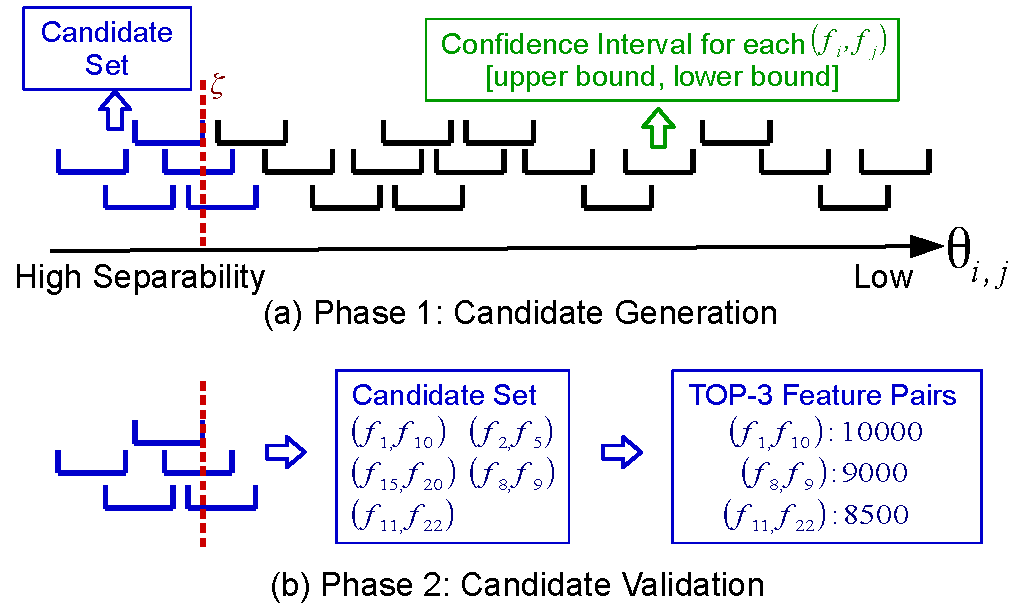
\includegraphics[width=\linewidth]{fig/sampling.pdf}
 \vspace{-9mm}
\caption{Phases of \sampling. (a) To calculate the \topthree feature pairs, the confidence interval of $\theta_{i,j}$ is calculated for all feature pairs evaluated on the sample set $\sss$ and a subset of candidates (blue intervals) are selected for validation. (b) The five selected candidates (center box) are evaluated on the whole object set $\hat{\oo}$ to compute the exact $\theta_{i,j}$ and pick the \topthree (rightmost box).}
\vspace{-5mm}
\label{fig:sampling}
\end{figure}

\stitle{Candidate Generation.} %\label{sssec:generate}
Let $\sss$ be a sample set drawn uniformly from the object set $\hat{\oo}$. Given a feature pair $(f_i,f_j)$, let $\theta_{i,j}(\sss)$ be the number of correctly separated objects in $\sss$. Let $\tilde{\theta}_{i,j}$ be the estimated separability score of all objects based on the sample set $\sss$. First, we can estimate $\tilde{\theta}_{i,j}$ from $\theta_{i,j}(\sss)$ using Equation~\ref{eqn:est_score} by assuming the ratio of correctly separated samples in $\sss$ is the same as that in $\hat{\oo}$.
\begin{equation}\label{eqn:est_score}
\tilde{\theta}_{i,j} = \frac{\theta_{i,j}(\sss)}{|\sss|} \cdot n
\end{equation}
\noindent Next, we show that with a constant sample set size $|\sss|$, $|\theta_{i,j}-\tilde{\theta}_{i,j}|$ is bounded by a small value with high probability, using Hoeffding's' inequality~\cite{hoeffding1963probability}. We formally quantize the sample set size in Theorem~\ref{them:est}.

\begin{theorem}[Estimation Accuracy]\label{them:est}
By considering $\Omega(\frac{1}{\epsilon^2}\cdot \log(\frac{1}{\delta}))$ samples, with probability at least $1-\delta$, we have $|\frac{\theta_{i,j}(\sss)}{|\sss|}-\frac{\theta_{i,j}}{n}| \leq \epsilon$, i.e., $|\tilde{\theta}_{i,j}-\theta_{i,j}|\leq \epsilon n$.
\end{theorem}

\begin{proof}
  Based on Hoeffding's inequality:
  $$Pr(|\frac{\theta_{i,j}(\sss)}{|\sss|}-\frac{\theta_{i,j}}{n}| \geq \epsilon) \leq 2e^{-2|\sss|\epsilon^2}$$
  Hence, when $|\sss| = \frac{1}{2\epsilon^2}\cdot \log(\frac{2}{\delta}) = \Omega(\frac{1}{\epsilon^2}\cdot \log(\frac{1}{\delta}))$, we have:
$$
  Pr(|\frac{\theta_{i,j}(\sss)}{|\sss|}-\frac{\theta_{i,j}}{n}| \geq \epsilon) \leq \delta \ \ \ \ \ \ \ \ \ \ \ \square
$$
\end{proof}
\noindent We can treat $\log(1/\delta)$ as a constant, e.g., by setting $\delta = 0.05$. Thus, Theorem~\ref{them:est} essentially states that with only $\Omega(\frac{1}{\epsilon^2})$ samples, with probability 95\%, the confidence interval for $\theta_{i,j}$ is $[\tilde{\theta}_{i,j}-\epsilon n, \tilde{\theta}_{i,j}+\epsilon n]$. Note that the sample size $|\sss|$ only depends on $\epsilon$ and is independent of the number of objects, $n$. Hence, the \sampling module helps \genviz scale to datasets with large $n$.
%For instance, when setting $\epsilon=0.05$, the sample size is fixed to be $400$.

With Theorem~\ref{them:est}, we can first calculate the confidence interval of $\theta_{i,j}$ for each feature pair $(f_i,f_j)$, as shown in Figure~\ref{fig:sampling}(a). Next, we compute the lower bound of $\theta_{i,j}$ for the \topk feature pairs, denoted as $\zeta$ as shown by the red dotted line in Figure~\ref{fig:sampling}(a). Finally, we can prune feature pairs away whose upper bound is smaller than $\zeta$. Accordingly, the candidate set $\cc$ corresponds to the feature pairs depicted by the blue intervals in Figure~\ref{fig:sampling}(a). These feature pairs $\cc$ will be further validated in phase two, i.e., candidate validation. Typically, $|\cc|$ will be orders of magnitude smaller than $m^2$, the original search space for all feature pairs.
%We will verify this later in our evaluations (Section~\ref{sec:exp}).

\begin{example}[Candidate Generation]
We illustrate phase one using Figure~\ref{fig:sampling}(a). Set $\epsilon = 0.05$ and $K=3$. We sample a subset of all objects and compute the confidence interval of $\theta_{i,j}$ for each $(f_i,f_j)$. Next, we obtain the $3^{rd}$ lower bound $\zeta$ (red dotted line) in descending order among all the confidence intervals. Finally, we designate all feature pairs whose upper bound is larger than the red dotted line as blue feature pair candidates $\cc$.
\end{example}

\stitle{Candidate Validation.} %\label{sssec:validate}
Since we only estimated the separability scores $\theta_{i,j}$ for our feature pair candidates in phase one, we re-evaluate all of the candidates generated from phase one to produce our final feature pair ranking. This phase two evaluation is performed using the whole object set $\hat{\oo}$. \sinha{are we using early termination and object ordering in phase two?} \silu{no. We tried both and found that early termination is not helping most of time since 1) the feature pair candidates, which perform well in phase 1, are indeed the ones that are hard to prune and 2) \earlyT incurs some overhead itself.} For each feature pair $(f_i,f_j)\in \cc$, we calculate the separability score $\theta_{i,j}$ and find the \topk feature pairs (Figure~\ref{fig:sampling}(b)).

\stitle{Enhancement by Candidate Ordering.} Recall that in Section~\ref{ssec:earlyT} we proposed an enhancement that allows us to terminate computation by cleverly manipulating the order of the objects; here we similarly found a way to reduce the running time by changing the order in which feature pair candidates are validated in phase two. Instead of directly validating each feature pair candidate, we first order the candidates in descending order according to the upper bound of each candidate's confidence interval. Then, we sequentially calculate the full separability score $\theta_{i,j}$ for each feature pair, and update $\zeta$ correspondingly. Recall that $\zeta$ is the current estimate of the lower bound of $\theta_{i,j}$ for the \topk feature pairs. Finally, we terminate our feature pair validation when the next feature pair's upper bound smaller than the current value of $\zeta$ (Figure~\ref{fig:candidate_ordering}).

\begin{figure}[h]
 \centering
 \vspace{-10mm}
 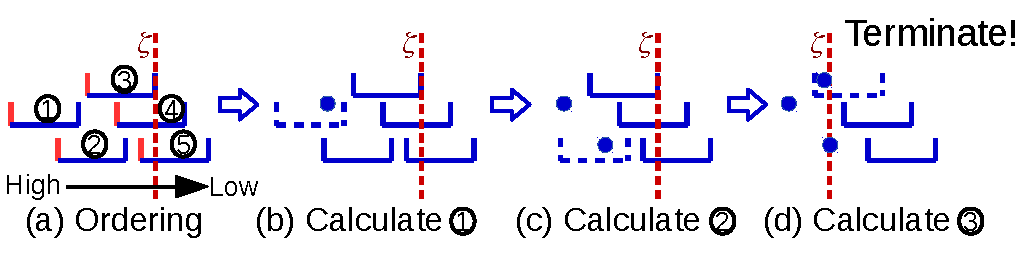
\includegraphics[width=\linewidth]{fig/candidate_ordering.pdf}
 \vspace{-8mm}
\caption{Enhancement by Candidate Ordering. (a) Feature pair candidates are sorted by the upper bounds of their confidence intervals (solid red boundary), and the lower bound of the \topthree feature pairs, i.e., $\zeta$, is set (red dotted line). (b,c,d) For each feature pair, we calculate $\theta_{i,j}$ (filled blue circle) using all objects and update $\zeta$ if necessary. Note that $\zeta$ is increased in (d) after evaluating the third feature pair and since $\zeta$ is larger than the upper bound of the fourth feature pair, candidate validation phase can terminate and return the top ranking feature pairs.}
\vspace{-5mm}
\label{fig:candidate_ordering}
\end{figure}

\sinha{ some readers will be confused by higher values being on the left}

%==================================================================
\subsubsection{Search Space Traversal} \label{ssec:traversal}

The optimizations discussed so far check fewer than $n$ objects for each feature pair and reduce the number of feature pairs for full evaluation in order to reduce the overall running time. Our \traversal module aims to reduce the number of feature pairs considered from $m^2$ to a smaller number.

\stitle{High Level Idea.} Instead of examining each feature pair, we only examine a limited number of feature pairs, but in an optimized traversal order. The number of examined feature pairs determines a trade-off between efficiency and accuracy. In general, fewer feature pairs checked will result in faster running times, though at the cost of accuracy in terms of the output.
The full search space for the feature pairs is the upper triangle in Figure~\ref{fig:traversal}(a), where each row represents $f_i$ and each column represents $f_j$. Let $\chi$ be the limit on the number of feature pairs to be examined. We propose two different traversal orders over the search space: horizontal and vertical, as follows:
\squishlist
\item \emph{Horizontal traversal (Figure~\ref{fig:traversal}(a)):} for each feature $f_i$, pair it with each other feature $f_j$, where $j\geq i$, to obtain $(f_i,f_j)$. Repeat for each $f_i$, where $1 \leq i\leq m$.
\item \emph{Vertical traversal (Figure~\ref{fig:traversal}(b)):} for each feature $f_j$, pair it with each other feature $f_i$, where $i\leq j$, to obtain $(f_i,f_j)$. Repeat for each $f_j$, where $1 \leq j\leq m$.
%\item \emph{Diagonal traversal (Figure~\ref{fig:traversal}(c)):} for a fixed value $v$, pair $(f_i,f_{v-i})$, where $1\leq i<v$. Repeat it for each $v$, where $2 \leq v\leq 2m$.
\squishend
\noindent
However, the traversal order does not convey any intuition if the feature set $\ff$ is in random order. Hence, we further propose to enhance \traversal by feature ordering in $\ff$.

\stitle{Enhancement by Feature Ordering.} We propose to first sort features based on single features' separability scores $\theta_{i,i}$. Single features with good separability individually are ranked higher. Let $\{f_1^{'} f_2^{'},\cdots,f_m^{'}\}$ be the sorted single-feature set. Next, we discuss the intuition behind the two different traversal order schemes. Consider partitioning the sorted single-feature list into three categories based on the single-feature separability score $\theta_{i,i}$: {\em good, average,} and {\em poor}.
\squishlist
\item \emph{Horizontal traversal:} the intuition is that there is at least one {\em good} or {\em average} single feature in each \topk feature pair $(f_i,f_j)$.
\item \emph{Vertical traversal:} the intuition is that both features in each \topk feature pair $(f_i,f_j)$ must be categorized as {\em good} or {\em average} individually.
%\item \emph{Diagonal traversal:}
\squishend
\noindent We examine the impact of these traversal schemes in our evaluations.

%The intuition behind horizontal traversal is that there is at least one {\em top} or {\em median} single features in the \topk feature pairs $(f_i,f_j)$; while the intuition behind horizontal traversal is that both features in \topk feature pairs $(f_i,f_j)$ must rank {\em top} or {\em median} by their own.

\begin{figure}[h]
 \centering
 \vspace{-5mm}
 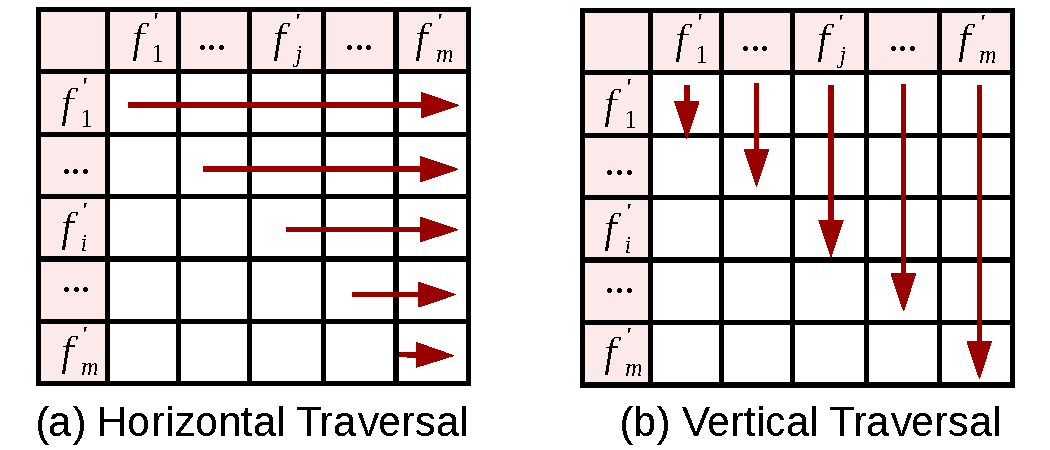
\includegraphics[width=0.85\linewidth]{fig/traversal.pdf}
 \vspace{-5mm}
\caption{\traversal Orderings. \genviz is able to examine the feature pair search space (a) horizontally or (b) vertically.}
\vspace{-5mm}
\label{fig:traversal}
\end{figure}

%Typically, $K$ is not large, e.g., {\sc Top-1000}, while $m$ is large, e.g., {\sc 20000}.
\begin{example}[\traversal]
Assume $m=2\times 10^4$. Initially, the number of possible feature pairs is roughly $\frac{m^2}{2}=2\times 10^8$. However, if we limit the number of considered feature pairs to $\chi=10^7$, we reduce our search space to $\frac{1}{20}$ of the total number of feature pairs. We order the single features by their individual separability scores. In horizontal traversal, only feature pairs with at least one individual feature ranked in the top 500 will be considered; while vertical traversal will consider only feature pairs with both individual features ranked better than 2000.
%the "worst" $f_i$ ranks around 500, while $f_j$ can be any feature in $\ff$. On the other hand, in vertical traversal, the "worst" $f_i$ (and $f_j$) ranks around 2000.
\label{examp:traversal}
\end{example}


%==================================================================
\section{Results}
\label{sec:exp}
In this section, we will illustrate that \genviz can rapidly identify meaningful feature pairs for the separability problem in real biological datasets to provide significant and interesting insights. First, we describe the datasets and algorithms used in our evaluations. Each algorithm that we evaluate represents a combination of optimization modules for ranking \topk feature pairs using our Rocchio-based separability measure. We report the running time and accuracy of the selected algorithms. Finally, we enumerate and visualize the \topk feature pairs returned by \genviz, compare them to the corresponding \topk single features, and examine their significance and support in existing publications.

%==================================================================
\subsection{Evaluation Setup}


\begin{table}[h]
\centering
%\vspace{-5mm}
\small
\begin{tabular}{|c|c|c|c|c|c|c|c|c|}
 \hline
 & $|\ff|$=$m$ & $|\oo|$=$N$ & $|\sss|$ & $\chi$ & \# of $\widehat{\oo}$ & avg($|\oo_+|$) & avg($|\oo_-|$) \\
 \hline
 \msig & 19,912 & 22,209 & 400 & $10^7$ & 10 & 295 & 21,914 \\
 \hline
 \lincs & 22,268 & 98,061 & 400 & $10^7$ & 40 & 165 & 97,897 \\
 \hline
 \end{tabular}
\caption{Dataset Statistics. For each dataset, the number of features $m$, objects $N$, sample size $|\sss|$ used by \sampling module, feature pairs $\chi$ examined by \traversal module, number of object sets: \# of $\widehat{\oo}$, average positive set size: avg($|\oo_+|$), and average negative set size: avg($|\oo_-|$).}
\label{tbl:dataset}
\vspace{-18pt}
\end{table}
\stitle{Datasets.} We conducted our tests on two different biological applications. In the first application, which we call \msig, we find pathways and other gene annotations that separate the differentially expressed genes from the undisturbed genes in specific cancer studies. In the other application, called \lincs, we find genes whose expression levels can distinguish experiments in which specific drug treatments were administered from others.

More specifically, in the \msig application, we are given a feature-object matrix with genes as the objects and different gene properties as the features. A natural way to construct this matrix is to define a collection of properties such as Gene Ontology terms~\cite{gene2014gene}, PFam domains~\cite{finn2015pfam}, and KEGG pathways~\cite{kanehisa2016kegg}, and use a binary representation to indicate whether each gene is known to have a property. This is equivalent to constructing a network with gene and property nodes, with edges representing known annotations, and recording adjacency information on each gene as its feature values. We generalized this notion of gene-property relationships by adding homology edges (connecting homologous gene pairs based on BLAST scores~\cite{altschul1990basic}) to the above network, and used the DRaWR algorithm~\cite{blatti2016characterizing} to perform a random walk with restarts on the heterogeneous network, thereby scoring the connectivity of each property node to each gene node. This resulted in the assignment of a numeric value for each gene-property pair ($g$, $r$), representing not only whether the gene is annotated with that property but also whether other genes closely related to gene $g$ are annotated with property $r$. We thus obtained a feature-object matrix describing each gene (object) as a vector of its strength of association with each property (feature) in light of prior biological knowledge.
%The values in this matrix correspond to the network connectivity between the node representing the feature gene set annotation and the node representing the object gene in a heterogeneous network of prior biological knowledge. To calculate these network connectivity scores we perform a random walk on the heterogeneous network that restarts at the feature gene set annotation node \needcite{DRAWR} and then observe the stationary probabilities of being at each gene node. The heterogeneous network here was constructed with information from BLAST, Gene Ontology, Pfam, and Pathway \needcite{each of these sources}.
\cb{still need to be certain on the steps required to create this matrix, also may want to mention restart prob, etc} The positive genes for each dataset in the \msig collection are the set of differentially expressed genes (DEGs) in a specific cancer study, as per Molecular Signatures Database~\cite{subramanian2005gene}. Each of our tests is an application of \genviz to such a dataset, reporting pairs of properties that separate DEGs of that cancer study (the ``positive'' set) from all other genes (the ``negative'' set).

In the \lincs application, the feature-object matrix contains expression values for different genes (features) across many drug treatment experiments (objects) conducted on the MCF7 cell line by the LINCS L1000 project~\cite{subramanian2017next}. The values of the matrix are gene expression quantities as reported by the ``level-4' imputed z-scores measured in the L1000 project. In each dataset, the positive object set includes multiple experiments that used the same drug, at varying dosages and for varying durations. We applied \genviz on each dataset so as to find the top pairs of genes (feature pairs) whose expression values separates the \lincs experiments relating to a single drug from all other \lincs experiments.

See Table~\ref{tbl:dataset} for further details of datasets used in the two applications just introduced. Note that the average number of positive objects in a dataset is far fewer than the average number of negative objects. In order to address this imbalance, we adjust Equation~\ref{eqn:s_line} to a weighted sum form as shown in Equation~\ref{eqn:s_line_weighted}.

\sinha{why did we chose the number of object sets, 10 and 40} \cb{this is an artifact of how we began. silu was going one or two \msig at the beginning and then expanded to 10 out of the ~50 that I created for Greg. For LINCS we started with 40 because those experiment sets were ones with >~100 samples}

%For each of the two applications, the numbers of features $m$, objects $N$, sample size $|\sss|$, and the examined feature pairs $\chi$ are shown in Table~\ref{tbl:dataset}. We tested on 10 different datasets for \msig and 40 different datasets for \lincs. For each positive object set, we treat all of the remaining objects as the negative set and list the average number of positive and negative objects in Table~\ref{tbl:dataset}.

\begin{equation}\label{eqn:s_line_weighted}
\hspace{3mm} \theta_{i,j}^{\ell}= \sum_{o_k\in{\oo_-}}{\theta_{i,j}^{\ell,k}}+\frac{|\oo_-|}{|\oo_+|}\cdot\sum_{o_k\in{\oo_+}}{\theta_{i,j}^{\ell,k}} %{\sf Separability \hspace{1mm} Score\hspace{1mm} with\hspace{1mm} Line\hspace{1mm} \ell:}
\end{equation}

%\stitle{Metrics.} We focus on two major metrics in our test: separability score and time. Specifically, each algorithm outputs $k$ feature pairs with highest separability score, i.e., \topk feature pairs, and we call the smallest separability score among the \topk feature pairs as \topk separability score.
%, where $m$ and $n$ are constants depending on the size of the feature-object matrix, $|\sss|$ and $\chi$ are the predetermined sampled set size and limit on the number of feature pairs considered, and $|\cc|$, the number of feature pair candidates is variable and is generated during the algorithm

\begin{table*}[t]
\centering
\small
\begin{tabular}{|c|c|c|c|c|c|c|c|c|}
 %\hline

 \hline
 & Transformation & \earlyT & Object Ordering & \sampling & Candidate Ordering & \traversal & Feature Ordering & Complexity\\
 \hline
 \baseline & yes & no & no & no & no & Any & no & $O(m^2n)$\\
 \hline
 %\early & yes & yes & no & no & no & Any & no & $O(m^2n)$\\
 % \hline
 \earlyOrder & yes & yes & yes & no & no & Any & no & $O(m^2n)$\\
 \hline
 \samp & yes & no & no & yes & no & Any & no & $O(mn+m^2|\sss|+|\cc|n)$\\
 \hline
 \sampOpt & yes & no & no & yes & yes & Any & no & $O(mn+m^2|\sss|+|\cc|n)$\\
 \hline
 \horiz & yes & no & no & yes & yes & Horizontal & yes & $O(mn+\chi|\sss|+|\cc|n)$\\
 \hline
 \vertic & yes & no & no & yes & yes & Vertical & yes & $O(mn+\chi|\sss|+|\cc|n)$ \\
 \hline
 \end{tabular}
\caption{Selected Algorithms Using Different Optimization Modules. For each algorithm (row), shows which optimization modules are employed and the running time complexity for that combination where $m$ and $n$ are the number of features and objects, $\sss$ is the sampled set size, $\chi$ is the limit on the number of feature pairs considered, and $\cc$ is the number of generated feature pair candidates.}
\label{tbl:alg}
\vspace{-18pt}
\end{table*}

\sinha{maybe naming algorithms A0, A1-A5.}
\sinha{describe table as tree?}
\agp{add approximate column}

\stitle{Algorithms.} In our evaluation, we experimented with six different selected combinations of the optimization modules introduced in Section~\ref{sec:opt}, as listed in Table~\ref{tbl:alg}. Other combinations that were not selected were always inferior to the ones shown, e.g., the unlisted algorithm with only \trans and \earlyT modules always has a worse running time and outputs the \topk feature pairs with the same separability score as the selected \earlyOrder combination. For our baseline, \agp{if we are using this for our baseline than I propose we discard its description if we are lacking in space...let's discuss} we use the algorithm with only the feature-object matrix pre-transformation optimization module (\trans). The last column in Table~\ref{tbl:alg} shows the running time complexity of different algorithms. Take \horiz as an example on how the running times are calculated. First, the \trans module takes $O(mn)$ time. \cb{ note, scoring single features takes O(mn) time and uses only transformation optimization.} Then, the \traversal module requires a sorting over the feature set, taking $O(m\log m)$\footnote{Since $m\log m < nm$, we omit term $m\log m$ from the overall complexity.} time. Finally, using the \sampling module over $\chi$ feature pairs, the running time is reduced from $O(m^2n)$ time to $O(\chi|\sss|+|\cc|n)$ time, where the first and second term represent the time for candidate generation and candidate validation respectively. Note that $|\cc|$ is typically orders of magnitude smaller than $\chi$ in \horiz, as discussed in Section~\ref{ssec:sampling}.

\stitle{Evaluation Setup.} We implemented the algorithms in C++, and conduct the evaluations on a machine with 16 CPUs and 61.9 GB of RAM.

%==================================================================
\subsection{Comparison of Different Algorithms}
\label{sec:exp_comp}

In this section, we first justify that Rocchio-based measure is a good proxy for the best possible separating score, i.e., $\theta_{i,j}$, computed by a brute force method Then we compare the performance of the various selected algorithms in terms of the running time and the separability scores of their \topthousand reported feature pairs.

\begin{figure}[h]
\centering %%% not \center
\vspace{-2mm}
\subfigure[Best Feature Pair Comparison]{\label{fig:brute_rocchio_ratio}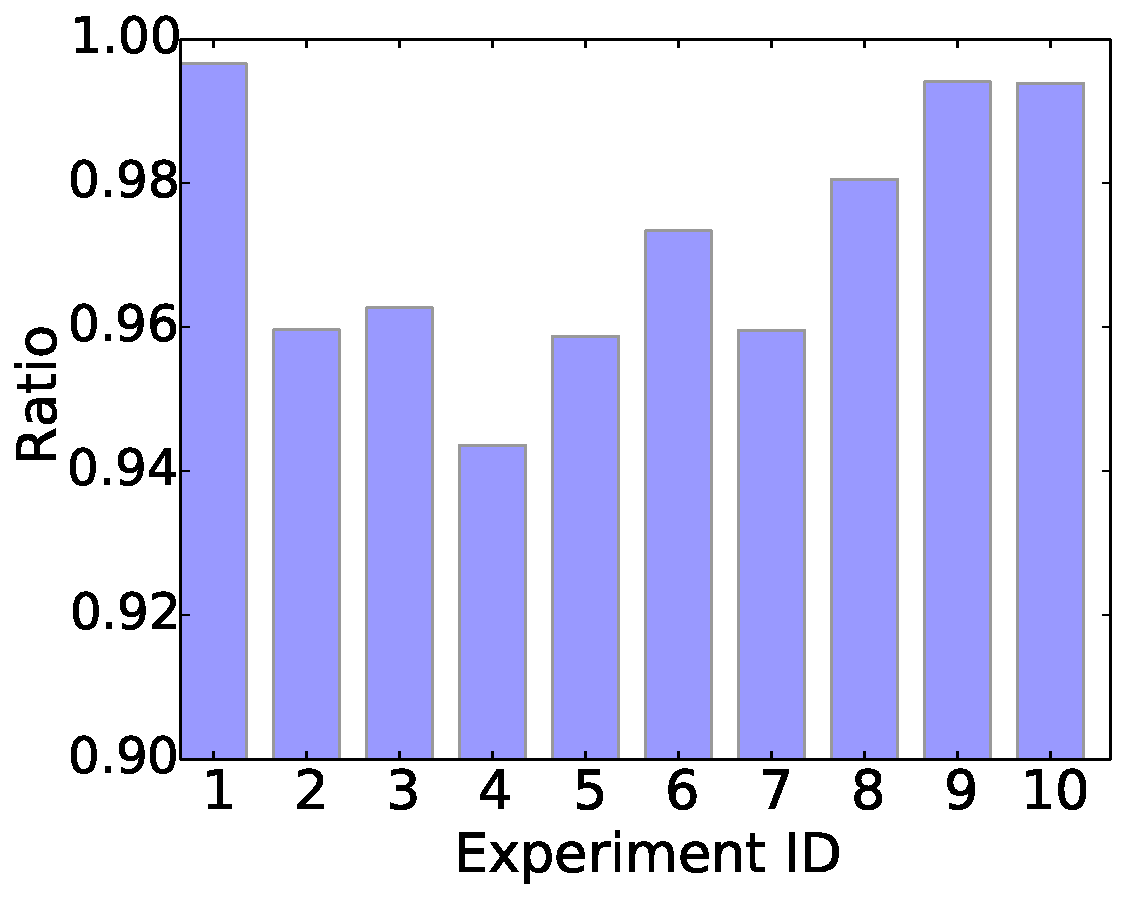
\includegraphics[width=.235\textwidth]{fig/rocchio_brute_ratio.pdf}}
\subfigure[Measure Comparison]{\label{fig:brute_rocchio_score}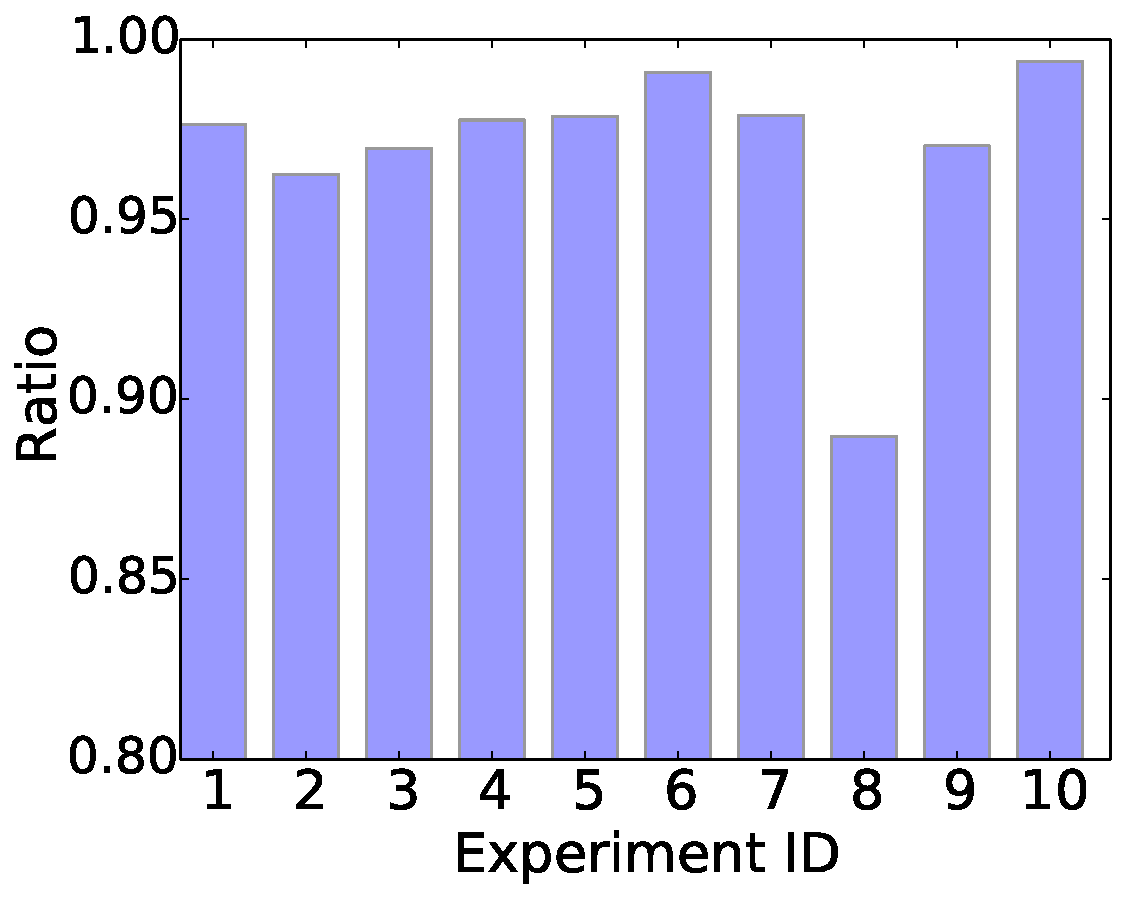
\includegraphics[width=.235\textwidth]{fig/rocchio_brute_score.pdf}}
\vspace{-5mm}
\caption{Comparison of Brute Force-based and Rocchio-based separability score. (a) For each of 10 datasets, we display the ratio of the true separability score between the best feature pair chosen by brute force and by the Rocchio-based method. (b) For each dataset, we display the ratio of the true separability score and the Rocchio-based separability score for the best feature pair selected using Rocchio-based method.}
\vspace{-5mm}
\label{fig:brute_rocchio}
\end{figure}

\stitle{Brute Force vs. Rocchio-based.} As we have discussed in Section~\ref{sec:metric}, when using brute force, we need to consider $O(n^2)$ lines in order to find the best separating line $\ell^* \leftarrow \arg_\ell \max \{\theta_{i,j}^{\ell}\}$, leading to a total running time complexity $O(n^2m^2)$ when considering all feature pairs. An alternative is to use Rocchio-based representative separating line $L$, dramatically reducing $O(n^2)$ lines considered to $O(1)$. Since the brute force method becomes computationally infeasible for datasets with large $n$, we compared the Rocchio-based measure to the brute force-based measure using
%a small $\widehat{\oo}$ for
the 10 datasets in \msig, for which the average number of positive objects was 295.
\sinha{Is the notation correct? Isnt 295 the average number of *positive* objects? } \cb{silu, I am also slightly confused. did we do the brute force comparison with pos vs neg msig or pos vs all msig?}
We call the brute force-based separability score the {\em true} separability score, since it examines all possible separating lines. We first find the best feature pair using Rocchio-based measure and the brute force based measure separately (potentially different feature pairs) and then calculate the ratio of the true separability scores of the Rocchio versus the brute force best feature pairs (Figure~\ref{fig:brute_rocchio_ratio}). We observe that the Rocchio-based method picks a best feature pair that has true separability score similar to the best pair picked by brute force, with the ratio of the two scores being better than 0.94 in all ten datasets. Second, for the best feature pair identified by Rocchio-based method, we calculate the ratio of the brute force-based separability score and Rocchio-based separability score (Figure~\ref{fig:brute_rocchio_score}), and find the difference to be small.
\agp{odd to have this here when this section is mostly about algo comparison. maybe bring it up later?}

\begin{figure}[h]
\centering %%% not \center
\vspace{-5mm}
\subfigure[\msig]{\label{fig:msig_time}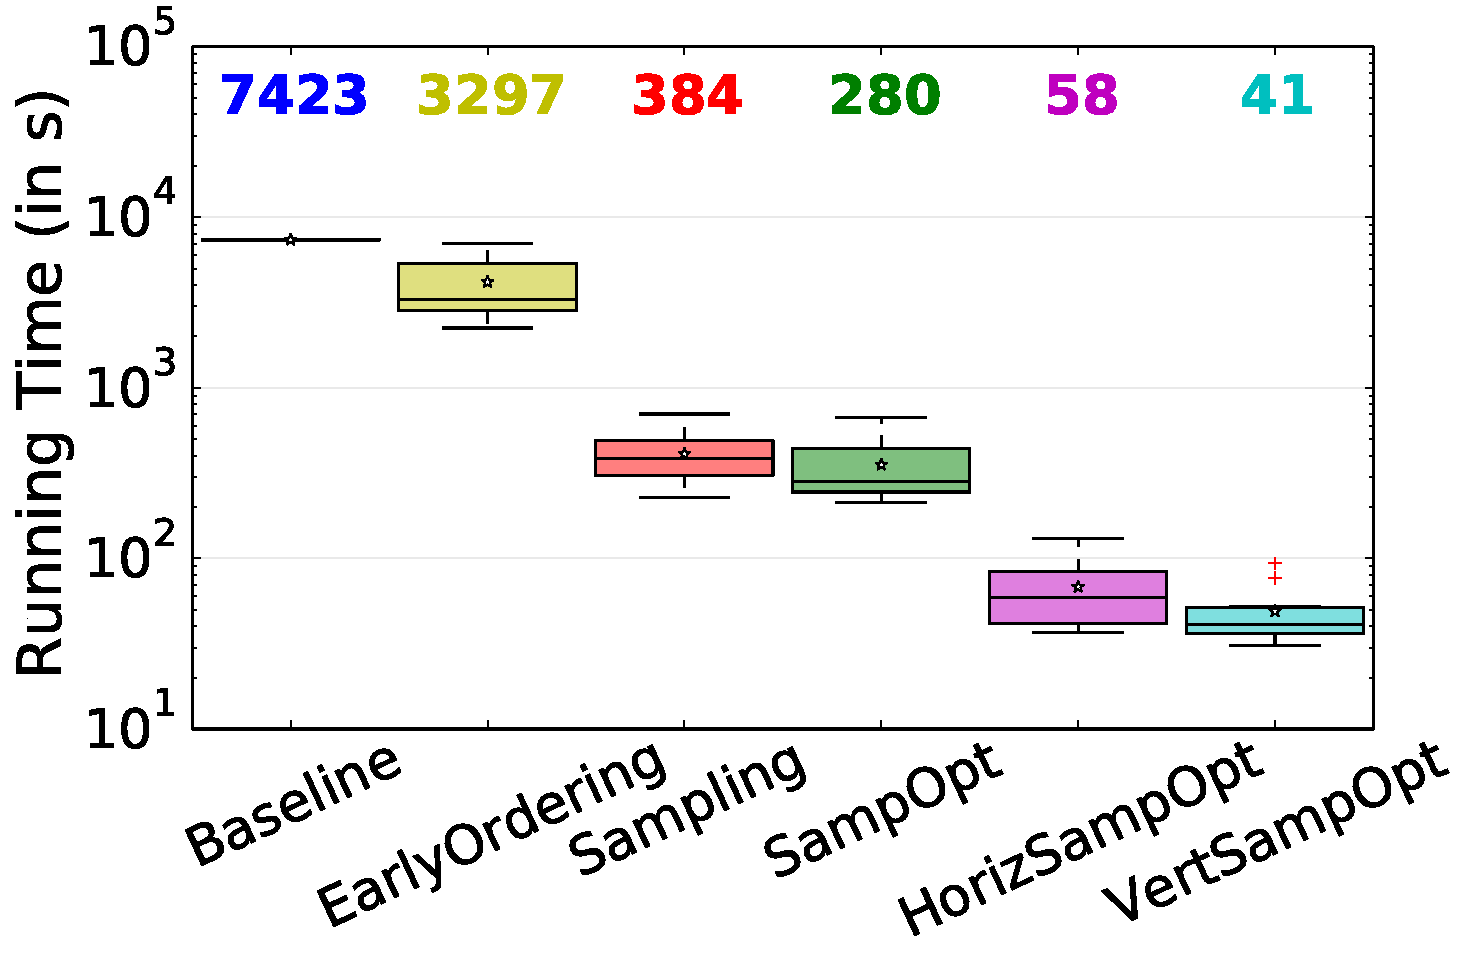
\includegraphics[width=.235\textwidth]{fig/msig_time.pdf}}
\subfigure[\lincs]{\label{fig:lincs_time}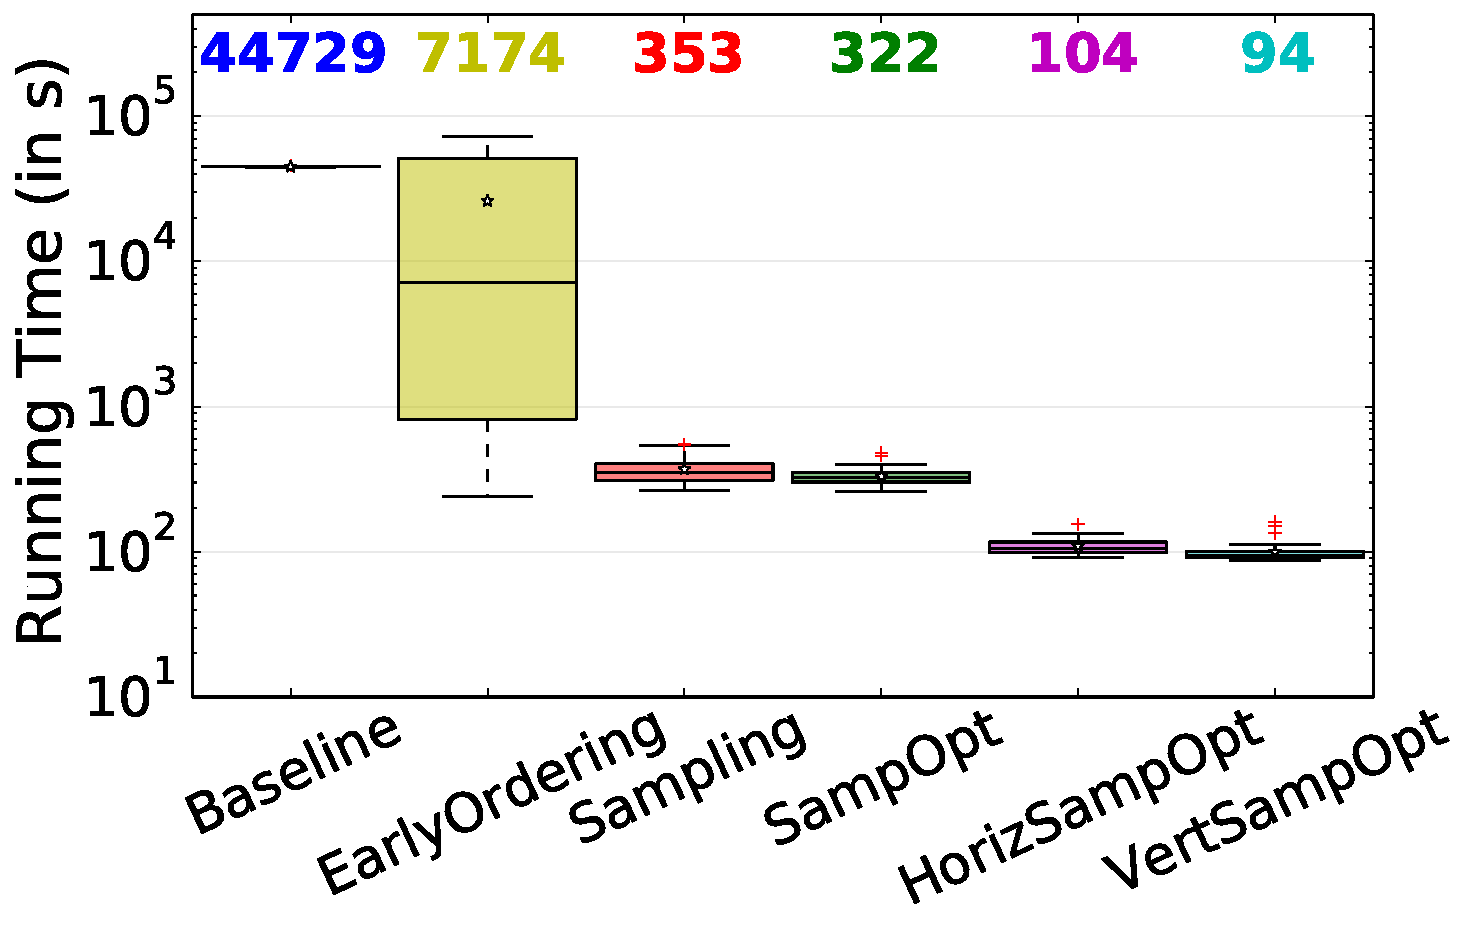
\includegraphics[width=.235\textwidth]{fig/lincs_time.pdf}}
\vspace{-5mm}
\caption{Running Time Comparison. A boxplot for each selected algorithm is shown with the median value appearing in matching color above. For each boxplot, whiskers are set to be $1.5\times$ the interquartile range, the outliers are shows as red dots, and the average is marked with as a black star. The number on the top shows the median running time for each algorithm.}
\vspace{-5mm}
\label{fig:time}
\end{figure}

\stitle{Running Time.} Figure~\ref{fig:time} depicts the running times of our different selected algorithms, as stated in evaluation setup. Each plotted box corresponds to one algorithm, representing the distribution of running times for finding the \topk feature pairs (by Rocchio score) for all datasets.
%(i.e., 10 gene set collections for \msig and 40 drug treatments for \lincs).

First, let us compare the median running times among different algorithms. For \msig, the \baseline takes more than 2 hours, \earlyOrder takes less than 1 hour, \samp and \sampOpt take around 6 and 5 minutes respectively, while \horiz and \vertic both take only 1 minute on average. Overall, the optimizations result in a reduction of the running time by over $180\times$. We next examine the effect of different modules on the running time. {\em (a) \earlyT:} we observe that the \earlyT module helps achieve a $2\times$ speed up, with the average number of checked objects (genes) reduced from $20K$ to $5K$ (Supplementary Table~\ref{tbl:supplement}); {\em (b) \sampling:} the \sampling module helps reduce the running time dramatically, with $20\times$ reduction from \baseline to \sampOpt, since on average only $2M$ candidates are generated from all possible $200M$ feature pairs (Supplementary Table~\ref{tbl:supplement});
{\em (c) \traversal:} the modules \horiz and \vertic achieve an additional $6\times$ speed-up compared to \sampOpt by terminating after only considering $\chi=10^7$ feature pairs, approximately $\frac{1}{20}$ (see Example~\ref{examp:traversal}) of all possible feature pairs. This speedup of \horiz and \vertic is approaching the limit set by the feature ordering overhead (around $6s$) and the time for the \trans module (around $8s$). (Supplementary Table~\ref{tbl:supplement}). The improvement over \sampOpt is not stronger because the candidate generation phase of \sampOpt is able to remove a vast number of the feature pairs from full evaluation that would be also be ignored by \horiz and \vertic (see Supplementary Table~\ref{tbl:supplement}).

Next, let us examine the log-scale interquartile range (IQR) of the running times for the different selected algorithms (Figure~\ref{fig:time}). We observe that \earlyOrder has the largest interquartile range, indicating that the \earlyT module used by this algorithm, which tries to reduce the number of objects evaluated for each feature pair, is very dependent on the object set and feature values. As we discussed in Section~\ref{ssec:earlyT}, \earlyT has no guarantee on improving the running time. In fact, the algorithm can occasionally be worse than the \baseline as shown in Figure~\ref{fig:lincs_time} because \earlyT incurs additional overhead for checking the criteria for pruning and early termination when scanning the object list for each feature pair.
\cb{we need more clarity (maybe in the discussion) why the early termination is included if it is not performing well, i.e. cases where we would recommend using it }

Similar results can be found in Figure~\ref{fig:lincs_time} for the \lincs application. Here, we observe over $400\times$ average decrease in the running time of finding the \topk feature pairs that separate the \lincs experiments of a single perturbagen from others. The greatest speedup comes with adding the \sampling module. In this setting, only $100K$ feature pair candidates, i.e., $|\cc|$, are checked out of all $250M$ feature pairs (Supplementary Table~\ref{tbl:supplement}). For the selected algorithms with best running times, \horiz and \vertic, the pre-transformation and feature ordering overhead account for an average of $45+35=80s$ of the overall 104 and 94 median seconds respectively.

% (b) the pruning of feature pairs in candidate generation phase is more powerful in \sampOpt, since on average the feature pairs considered in \horiz and \vertic is better than that in \sampOpt intuitively.


\begin{figure}[h]
\centering %%% not \center
\vspace{-5mm}
\subfigure[\msig]{\label{fig:msig_separability}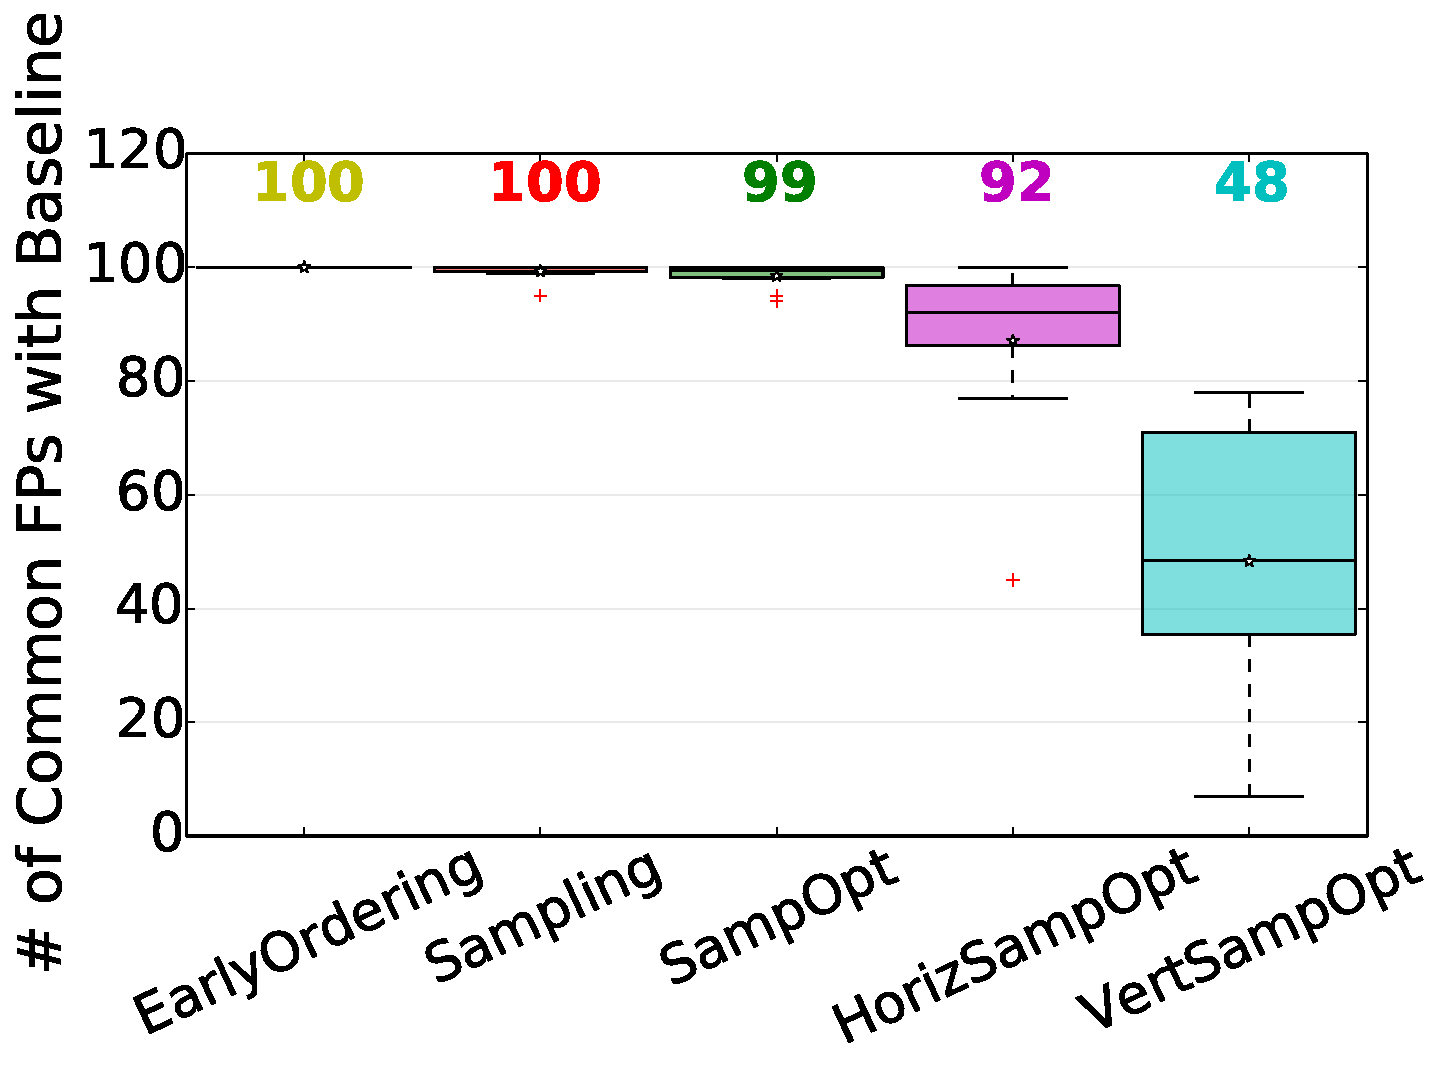
\includegraphics[width=.235\textwidth]{fig/msig_accuracy.pdf}}
\subfigure[\lincs]{\label{fig:lincs_separability}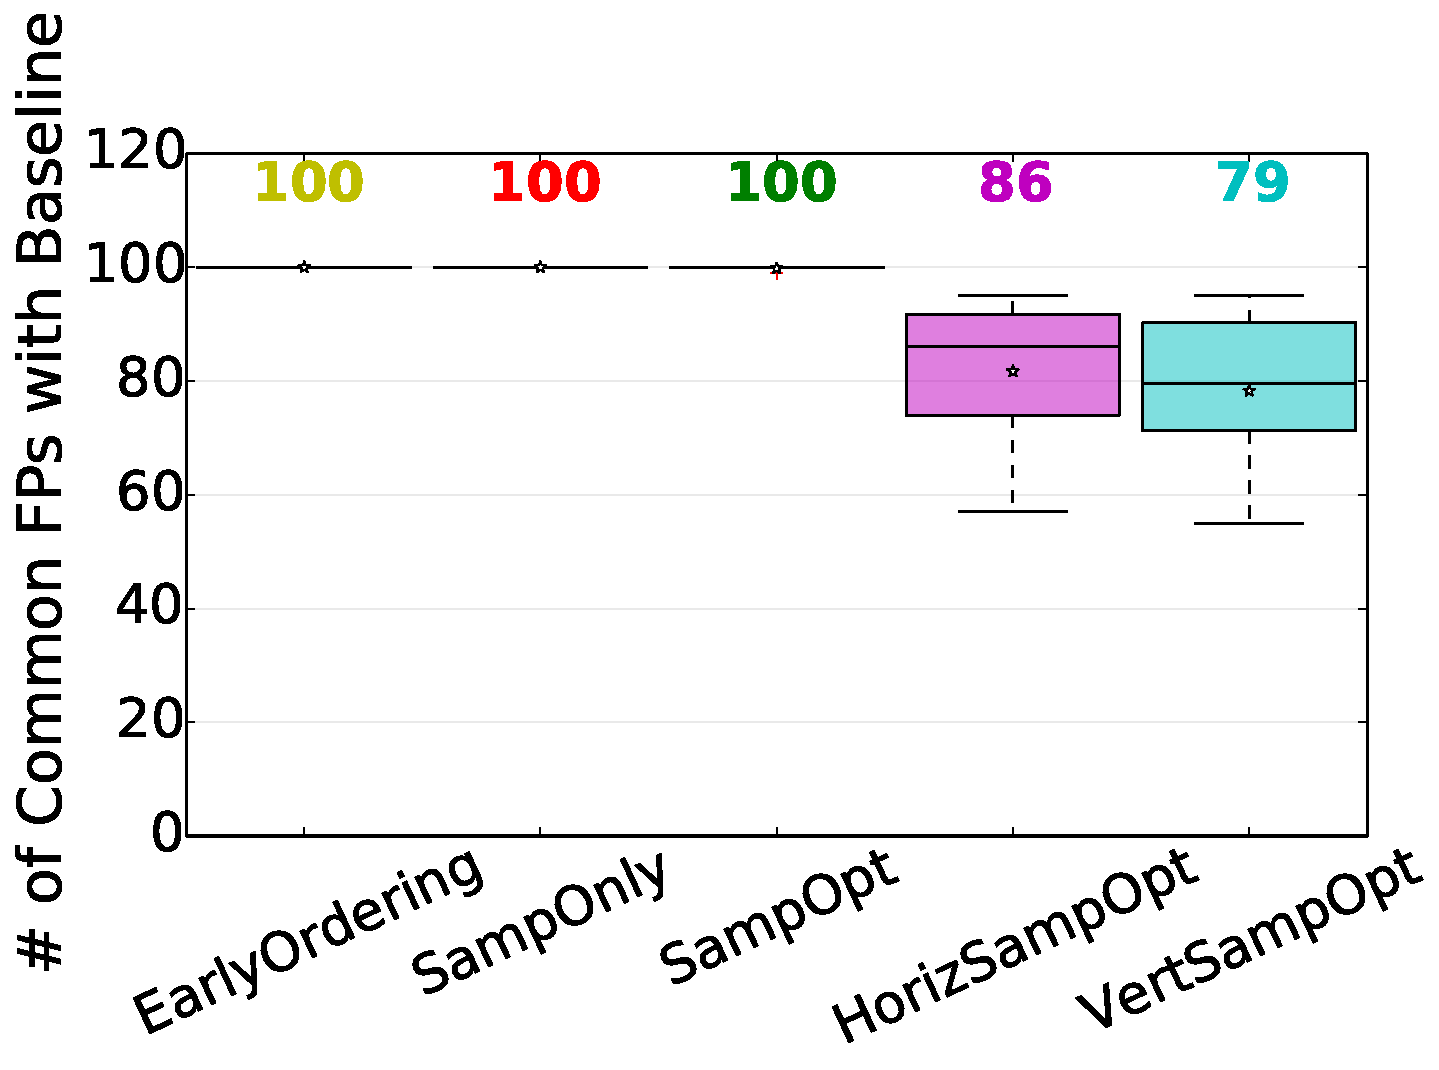
\includegraphics[width=.235\textwidth]{fig/lincs_accuracy.pdf}}
\vspace{-5mm}
\caption{Separability Quality Comparison. Boxplots in the style of Figure~\ref{fig:time} comparing the number of feature pairs each method returned from the 100 best feature pairs of the Baseline method.}
\vspace{-5mm}
\label{fig:separability}
\end{figure}

\sinha{alignment of algorithm names not ok in figure}

\stitle{Separability Quality.} Recall that the \earlyT module is a deterministic optimization and will produce the same \topk feature pairs as the baseline method. The \sampling module, on the other hand, is stochastic and places a probabilistic guarantee on the separability score of the feature pairs and therefore can only provide an approximate estimate of the \topk feature pair ranking. Finally, the \traversal module is heuristic and may output \topk feature pairs that are very different from the ranking produced by the \baseline algorithm. Since \baseline returns the true Rocchio-based separability score of each feature pair, we measured the quality of each selected algorithm by counting the number of common feature pairs returned in the \tophundred between the \baseline and the given algorithm. Figure~\ref{fig:separability} shows this separability quality comparison. Let us first focus on the \msig application. \earlyOrder, as expected, has exactly the same separability quality as the \baseline. We also observe that the \samp and \sampOpt rankings are nearly identical to the \tophundred feature pairs of the \baseline, owing to the probabilistic guarantee as stated in Theorem~\ref{them:est}. The \horiz and \vertic algorithms output a median of 92 and 48 feature pairs in common with \baseline, respectively, because of the heuristic \traversal module. In the \msig results, \horiz performs much better than \vertic, with the median much higher and the interquartile range much narrower, as shown in Figure~\ref{fig:msig_separability}. This suggests, as we hypothesized, that interesting separating feature pairs exist outside of only the combinations of the top single features as in \vertic. We repeated this quality analysis for the \lincs application and found that the \sampling based algorithms returned identical \tophundred feature pairs for all 40 datasets. The quality of the \traversal based algorithms was again lower, though there the separation in the performance of the \horiz and the \vertic algorithms was not as large as for the \msig application.

\stitle{Takeaways.} If the accuracy is paramount to the user, \sampOpt is the suggested algorithm; while if the running time is paramount to the user, \horiz is the desired algorithm.

%The p-value from Fisher's exact test represents the significance of deviation from the null hypothesis, i.e., the predicted label is independent of the real label. This significance test is frequently used to characterize gene sets \needcite{}.

%==================================================================
\subsection{Feature Pair vs. Single Feature.}\label{sec:FPvSF}

In this section, we quantify how statistically significant the top ranking results of the selected algorithms are. We show that we are often able to find separating feature pairs that are more significant than the best single separating feature. In order to assess the significance of a separating feature or feature pair, we first calculate the p-value using the one-sided Fisher's exact test on a $2\times2$ contingency table. This contingency table is constructed with the rows being the true positive and negative labels, the columns being the predicted positive and negative labels, and the values being the number of objects that belong to each table cell. Using the Fisher's exact test p-value, we assert that feature pairs can provide better separability performance or new insights compared to single features, i.e., (a) feature pairs have stronger p-values compared to the corresponding individual features even after the appropriate multiple hypothesis correction and (b) there exist high-ranked pairs of features that are poorly-ranked on their own as single features.

\begin{figure}[h]
\centering %%% not \center
\vspace{-5mm}
\subfigure[\msig]{\label{fig:msig_singleF}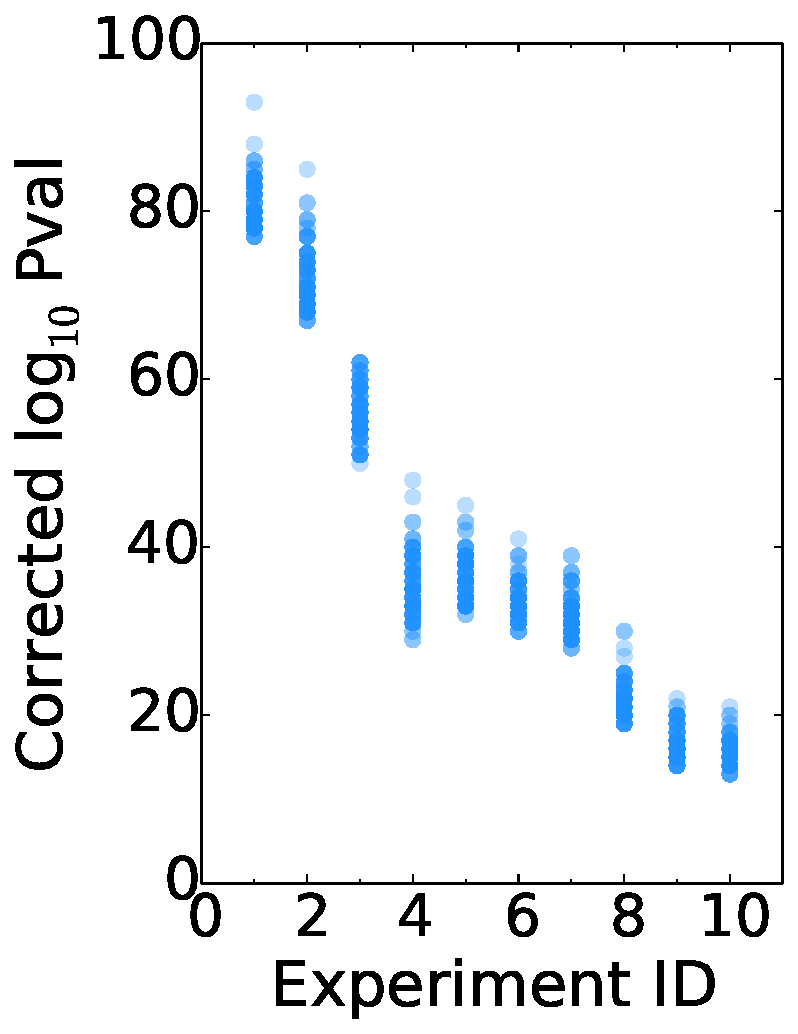
\includegraphics[width=.16\textwidth]{fig/msig_singleF.pdf}}
\subfigure[\lincs]{\label{fig:lincs_singleF}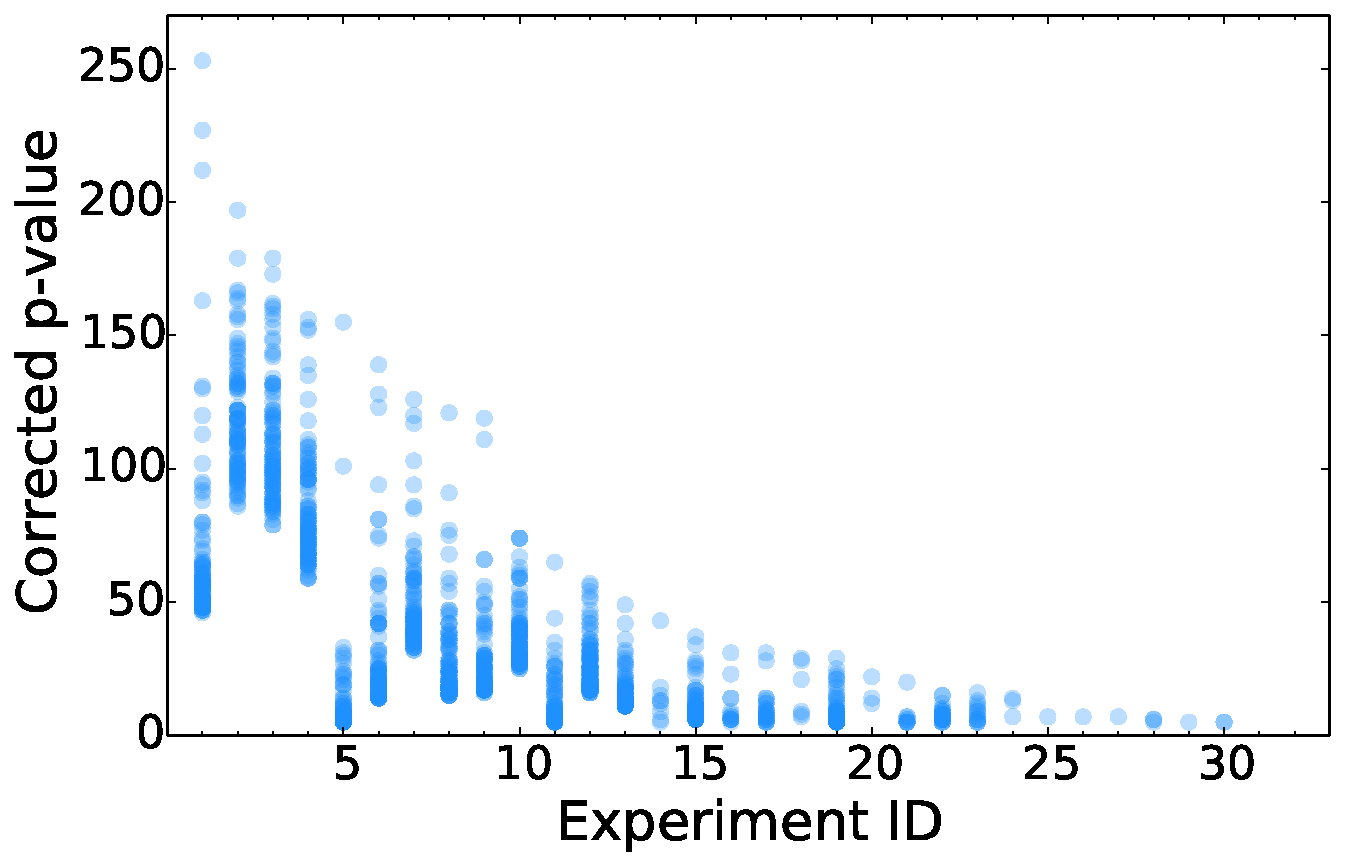
\includegraphics[width=.31\textwidth]{fig/lincs_singleF.pdf}}
\vspace{-5mm}
\caption{Single Feature Corrected P-value Distribution \sinha{Experiment ID -> Dataset ID}. For each experiment (x-axis), shows the significance ($-\log_{10} (corrected\_pval)$) of the \tophundred best single features (blue dots) for the (a) \msig and (b) \lincs datasets. We order the datasets by their best corrected single feature p-value, and discard the datasets where no single feature has corrected p-value better than $10^{-5}$.}
\vspace{-5mm}
\label{fig:singleF}
\end{figure}


\stitle{Single Feature.} Finding \topk single features is a special case of finding feature pairs by setting $i=j$, as noted in Section~\ref{ssec:trans} and Equation~\ref{eqn:s_object_transform_single}. For each single feature obtained, we compute the p-value with Fisher's exact test, denoted as $pval$. Next, we define the Bonferroni corrected p-value as $corrected\_pval= pval\times m \times n$, since there are $m \times n$ possible hypotheses, one for each possible single feature and separating line. We say a selected feature is significant if the corrected p-value is smaller than the threshold $10^{-5}$, i.e., $-\log_{10} (corrected\_pval)\geq5$. In Figure~\ref{fig:singleF}, we plot the distribution of the corrected p-value of the \tophundred features reported for each dataset in \msig and \lincs. We observe that 10 out of 10 datasets in \msig and 32 out of 40 datasets in \lincs have at least one significant single feature. We will focus on these 10 runs in \msig and 32 datasets in \lincs for the remainder of the paper. We observe very small p-values, $\leq 10^{-50}$, in the left part of Figure~\ref{fig:msig_singleF} and \ref{fig:lincs_singleF}, indicating a very strong relationship between the predicted and true object labels. This shows the effectiveness of linear separability and the Rocchio-based separability metric in identifying features that predict the different classes of objects.

%
%This shows the effectiveness of our Rocchio-based

\begin{figure}[h]
\centering %%% not \center
\vspace{-5mm}
\subfigure[\msig]{\label{fig:msig_FP}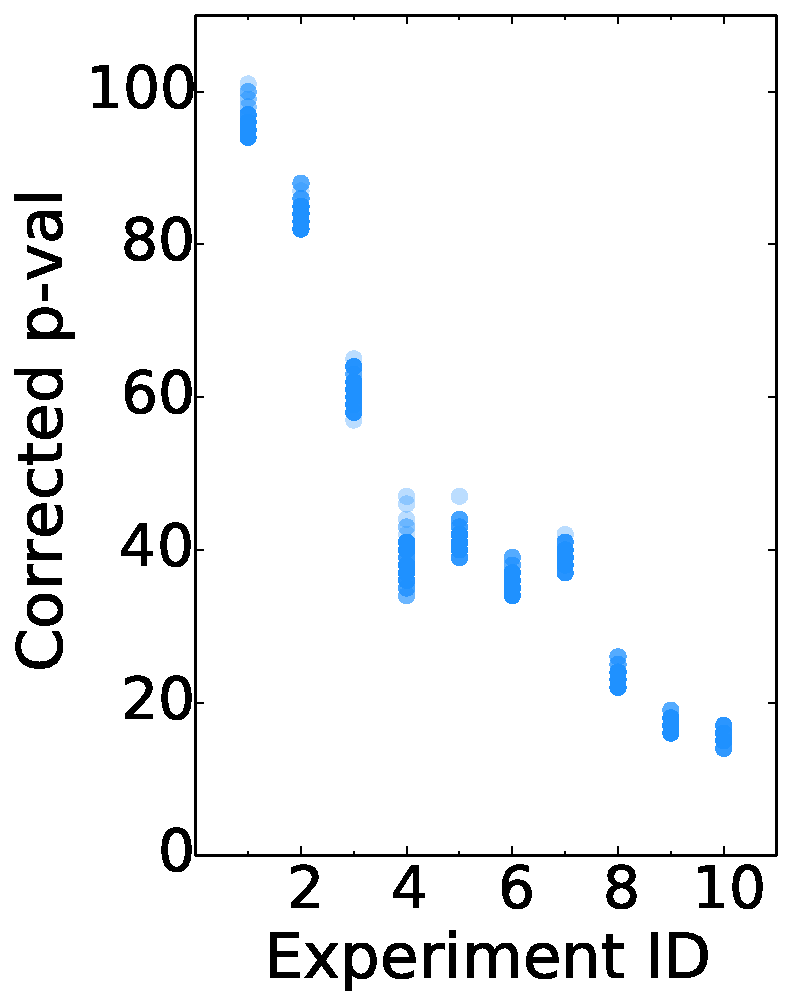
\includegraphics[width=.16\textwidth]{fig/msig_FP.pdf}}
\subfigure[\lincs]{\label{fig:lincs_FP}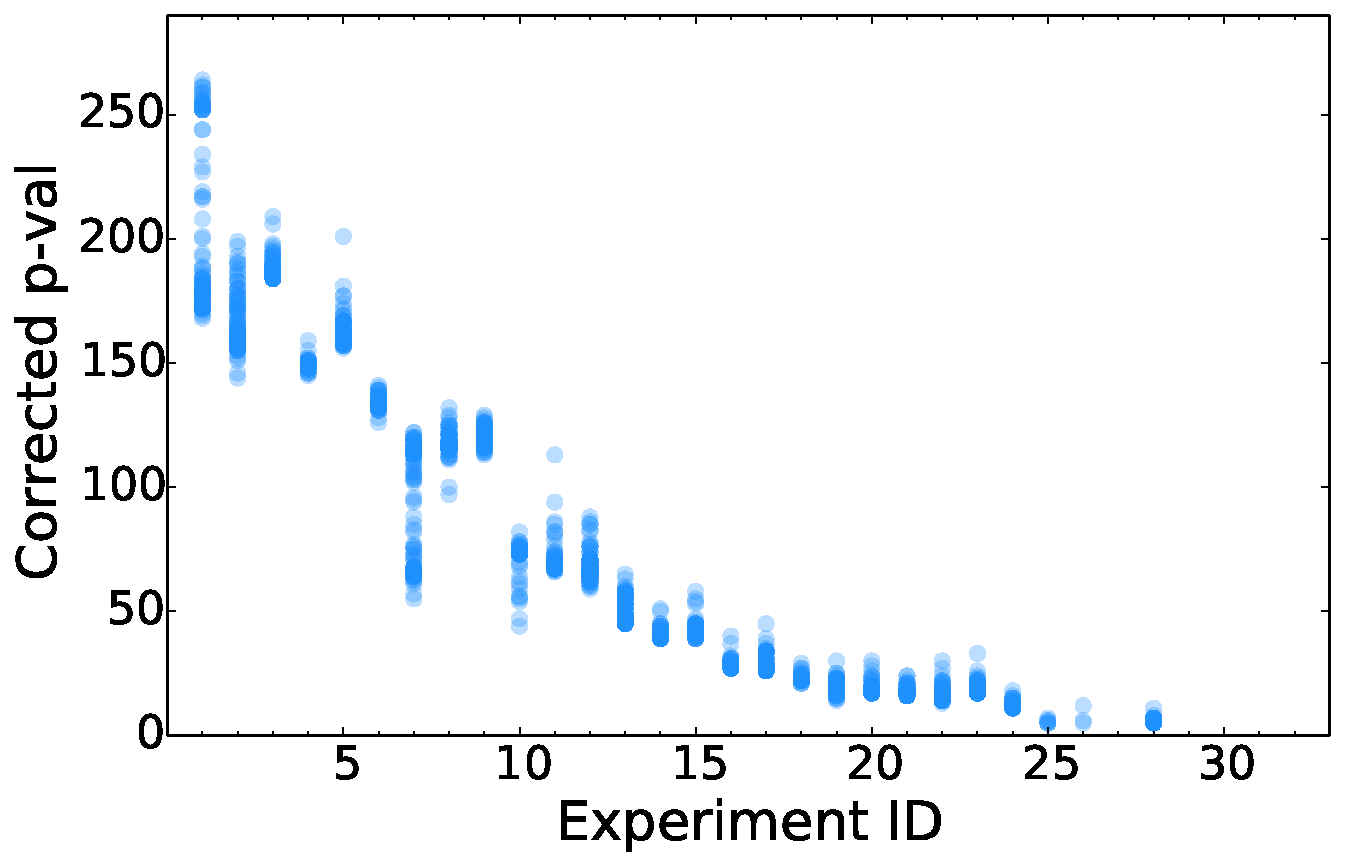
\includegraphics[width=.31\textwidth]{fig/lincs_FP.pdf}}
\vspace{-5mm}
\caption{Feature Pairs' Corrected P-value Distribution. Plotted significance for the \tophundred best feature pairs (blue dots) for each experiment in the (a) \msig and (b) \lincs datasets.}
\vspace{-5mm}
\label{fig:FP}
\end{figure}

\stitle{Feature Pair.} We next build the contingency tables and calculate the p-value for the \topk feature pairs. To correct for $m^2$ possible feature pairs and the $n^2$ possible ways to choose the separating lines for each feature pair, we apply a Bonferroni p-value correction to produce the $ corrected\_pval = pval\times m^2 \times n^2$. We plot the distribution of these corrected p-value for the \topk feature pairs in Figure~\ref{fig:FP}. Once again, the threshold for defining a significant feature pair is set to $10^{-5}$. We find that 10 out of 10 datasets in \msig and 27 out of 40 datasets in \lincs have at least one significant feature pair by this metric. Visual comparison of the \tophundred single features (Figure~\ref{fig:singleF}) to the \tophundred feature pairs (Figure~\ref{fig:FP}) per dataset reveals several datasets where the
corrected p-values of the feature pairs are more significant than those of the best single features, even after accounting for the larger search space. Admittedly, this is not always the case, e.g., for five \lincs datasets no feature pair was found to be significant at $ corrected\_pval \leq 10^{-5}$ while at least one single feature did meet this threshold. Overall, this analysis suggests that rapid discovery of top feature pairs may identify more significant patterns in the given dataset than a traditional single-feature analysis does.
%, we observe that the corrected p-values of the feature pairs are often more significant and more tightly \sinha{this is not necessarily convincing. Could be fp's that share a feature.} distributed than the single feature corrected p-values. This indicates
%that the best feature pairs have better separability quality than the top ranking single features even after accounting for the larger search space. \sinha{What about the \lincs datasets for which no significant feature pair comes out?}
In the following, we further illustrate that feature pairs can also provide better and new insights compared to single features.

\begin{figure}[h]
\centering %%% not \center
\vspace{-3mm}
\subfigure[\msig]{\label{fig:msig_histogram_diff}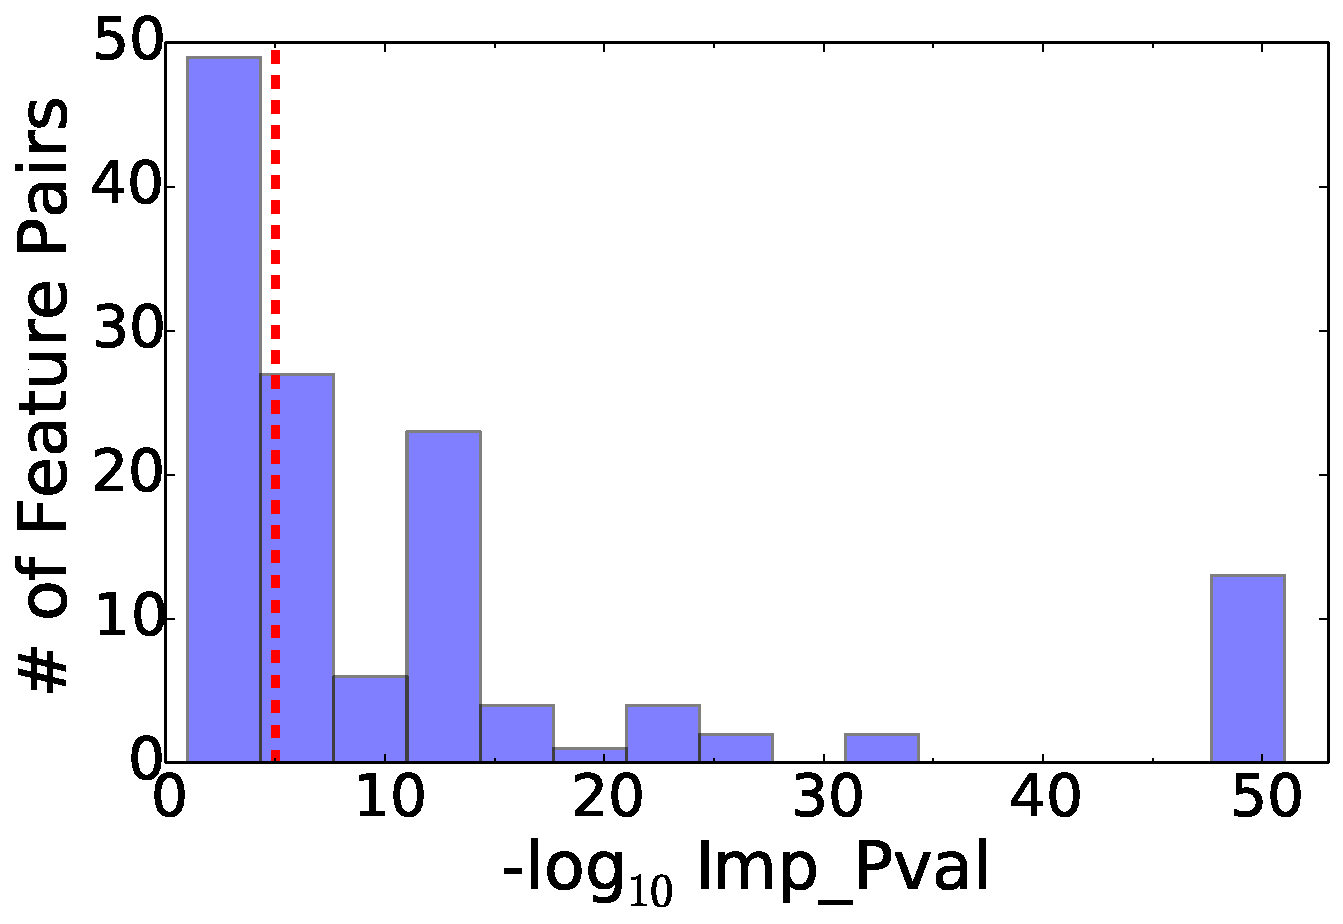
\includegraphics[width=.235\textwidth]{fig/histogram_msig_diff_pval.pdf}}
\subfigure[\lincs]{\label{fig:lincs_histogram_diff}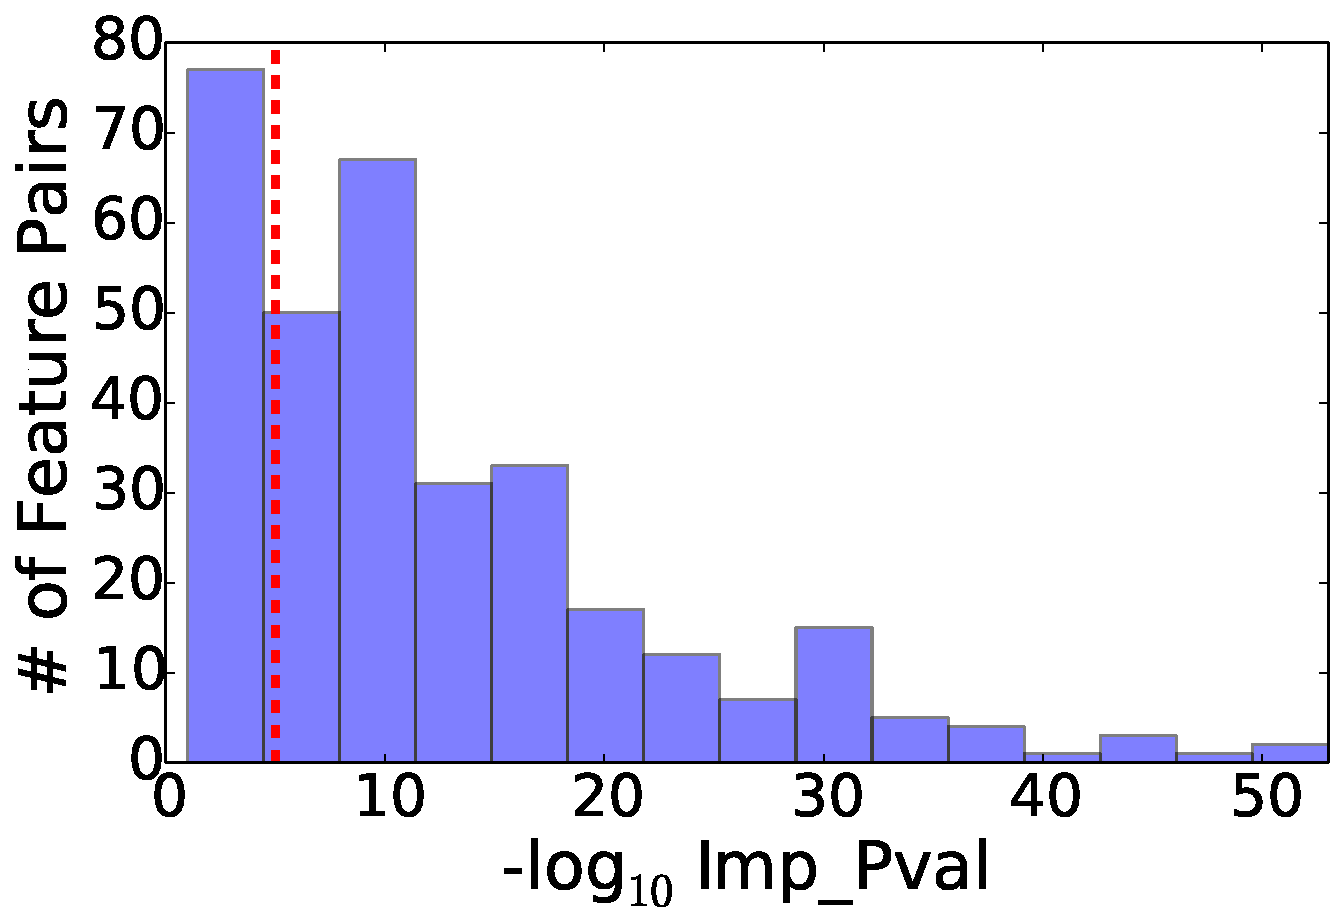
\includegraphics[width=.235\textwidth]{fig/histogram_lincs_diff_pval.pdf}}
\vspace{-5mm}
\caption{Histogram of $improv\_quot$. For the \toptwenty feature pairs from all runs from the (a) \msig and (b) \lincs datasets, distribution of the improvement of the feature pair significance over the corresponding single feature significance. The red line shows the significance threshold of 5.}
\vspace{-5mm}
\label{fig:histogram_diff}
\end{figure}

%Remember that the correction factors for single feature and feature pair are different: $mn$ vs. $m^2n^2$.

\stitle{Improvement from Single Feature to Feature Pair.} We have computed the corrected p-value for each single feature and feature pair. Now let us examine the improvement of each feature pair from its two corresponding single features in terms of p-value. For each feature pair $(f_i,f_j)$, we define the improvement quotient \xsinha{can we call improved p-value something else? It is grammatically incorrect. Not sure what though.} as the ratio between the corrected p-value of $(f_i,f_j)$ and the better of the corrected p-value of $f_i$ or $f_j$, i.e., $improv\_quot = \frac{corrected\_pval(f_i,f_j)}{\min(corrected\_pval(f_i),corrected\_pval(f_j))}$. In this set of results, we will focus on \toptwenty feature pairs for each dataset to improve the clarity of the presentation. In Figure~\ref{fig:histogram_diff}, we plot the histogram of $improv\_quot$ for 10 runs in \msig and 32 runs in \lincs. In both datasets, there are many feature pairs (to the right of the red dotted line) in the top 20 that are more significant than their corresponding single features, e.g., on average 8 among \toptwenty feature pairs with $-\log_{10} improv\_quot > 5$ for \lincs. This shows that there is a improvement from single features to some feature pairs in terms of the separability significance, at least for several datasets in our evaluations. In the next section, we will more carefully explore improved feature pairs like these commenting on their redundancy, reliability, and relevance. \xsinha{note here about possibility of redundant feature pairs contributing to the histogram.}


% \begin{figure}[h]
% \centering %%% not \center
% \subfigure[\msig]{\label{fig:msig_FP}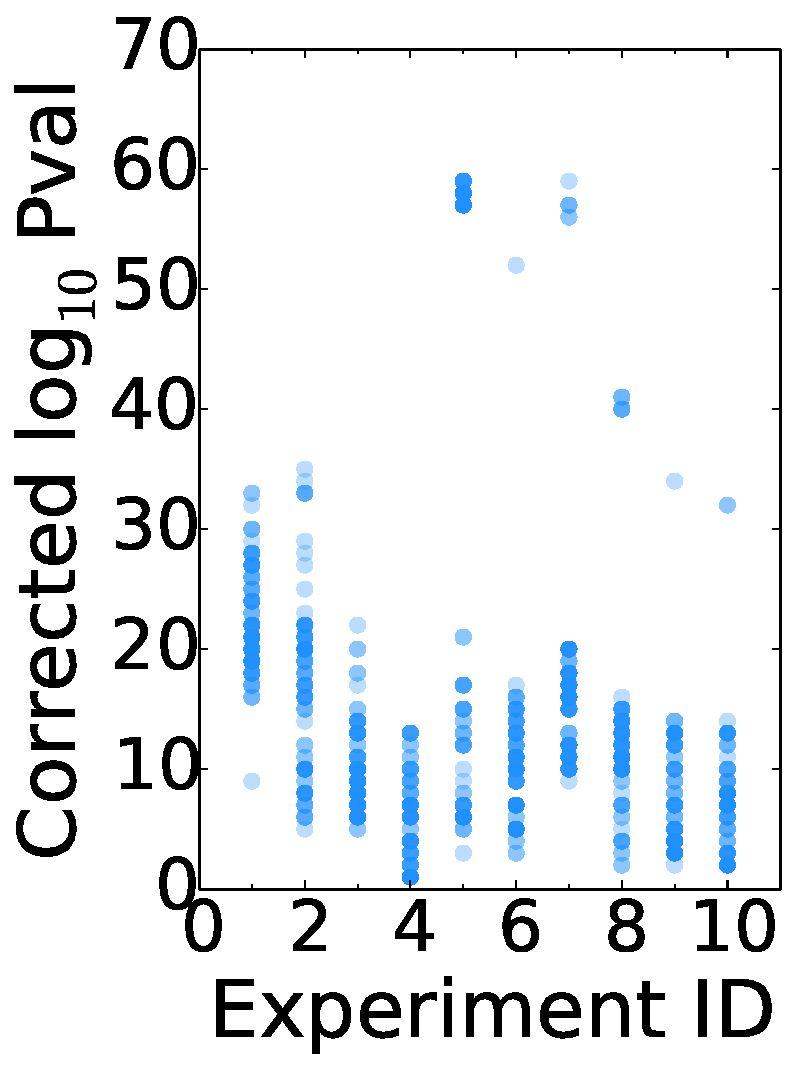
\includegraphics[width=.16\textwidth]{fig/msig_diff_pval.pdf}} # \tophundred
% \subfigure[\lincs]{\label{fig:lincs_FP}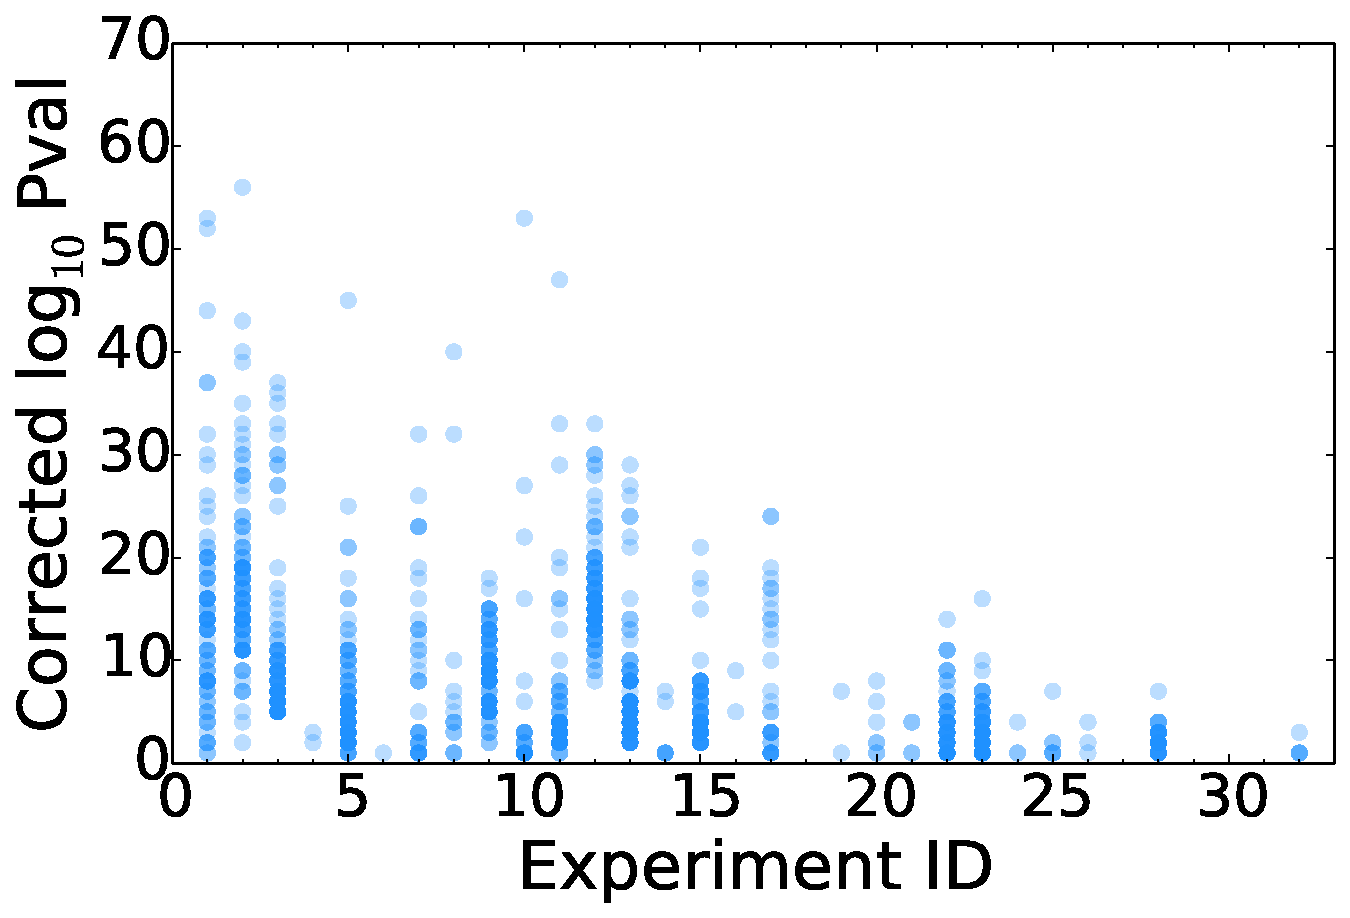
\includegraphics[width=.31\textwidth]{fig/lincs_diff_pval.pdf}}
% \caption{Top-100 Feature Pairs' Corrected P-value Distribution}
% \label{fig:FP}
% \end{figure}

\stitle{New Insight from Feature Pairs.} In order to assess the quality of the top ranking feature pairs, we focused on the \lincs data set where the objects were experimental treatments on the MCF7 breast cancer cell line with the same {\em drug} and the features were expression values for different {\em genes}. For the evaluations above, we used object sets for the 40 drugs with the largest number of LINCS experiments. For the following analysis, we refine our list to common drugs
\sinha{how did you arrive at this designation Charles?} \cb{this is done by manually looking at the list and flagging ones with short, common names based on lincs description that were in multiple databases}
and have at least 60 LINCS experiments on the MCF7 cell line. These nine drugs are vorinostat, trichostatin, estradiol, tamoxifen, doxorubicin, gemcitabine, daunorubicin, idarubicin, and pravastatin. For each chosen drug, we ran the \sampOpt algorithm of \genviz to rank the \topthousand feature (gene) pairs for separating the LINCS experiments of the drug from all other MCF7 experiments.

For all drugs, except pravastatin, all of the \topthousand ranked feature pairs were found to be significant ($-\log_{10} corrected\_pval > 5$). The average log significance of the \topthousand feature pairs correlated with the number of experiments ($r=0.91$) in the drug's positive object set (see Table~\ref{tbl:selected_fps}), suggesting that \genviz algorithms requires a minimum number of example objects to learn a meaningful separator between the two classes. \sinha{I dont see this as the suggestion/inference. This is expected because p-values for data from the alternative hypothesis tend to be smaller for greater sample sizes.} As described in the Section~\ref{sec:FPvSF}, we are especially interested in feature pairs where its corrected p-value is better than the corrected p-values of its corresponding single features ($-\log_{10} improv\_quot > 0$). We found 1070 "improved" feature pairs with improved separability over their single feature among the top1000 of these evaluation drugs sets. One drug, trichostatin, had especially strong performing single features and showed no feature pairs that significantly improved on them. The remaining seven drugs, however, benefited from the feature pair analysis and had as few as 9 (tamoxifen) and as many as 369 (doxorubicin) improved feature pairs (Table~\ref{tbl:selected_fps}). \xsinha{revisit this sentence. Doesnt make sense.}

\begin{table}[t!]
\centering
\small
\begin{tabular}{|l|c|c|c|c|}
\hline
 Drug & NumExprs & Avg Signif & Top1000 Signif & Top1000 Improved\\
\hline
vorinostat & 904 & 235.5 & 1000 & 287\\
\hline
trichostatin & 689 & 277.1 & 1000 & 0\\
\hline
estradiol & 325 & 166.8 & 1000 & 203\\
\hline
tamoxifen & 122 & 105.8 & 1000 & 9\\
\hline
doxorubicin & 104 & 28.0 & 1000 & 369\\
\hline
gemcitabine & 97 & 52.5 & 1000 & 116\\
\hline
daunorubicin & 91 & 40.9 & 1000 & 28\\
\hline
idarubicin & 78 & 30.1 & 1000 & 58\\
\hline
pravastatin & 61 & -7.5 & 0 & 0\\
\hline
Grand Total & & 43.1 & 9068 & 1070\\
\hline
 \end{tabular}
\caption{For each chosen drug from \lincs, the number of experiments in MCF7 cell line that were performed with that drug (NumExprs), and statistics for the top1000 feature pairs for that drug including the average $-\log_{10} corrected\_pval$ (Avg Signif), number of feature pairs with $-\log_{10} corrected\_pval > 5$ (Top1000 Signif), and number with $-\log_{10} improv\_quot > 0$ (Top1000 Improved).}
\label{tbl:selected_fps}
\vspace{-18pt}
\end{table}


Many of the above-mentioned 1070 significantly improved feature pairs are partially redundant, in the sense that they comprise a common best-ranked single feature (gene). An example of this is with the object set for the drug (compound) estradiol. We found the gene PRSS23 as the single feature with the highest separability and many feature pairs containing PRSS23 and a second gene as having an improved corrected p-value, for example (PRSS23, RAP1GAP), (PRSS23, TSC22D3), and (PRSS23, BAMBI). We looked for evidence of the relationship between the drug estradiol and these feature pair genes in the Comparative Toxicogenomics Database~\cite{grondin2018accessing} (CTD) and with our own literature survey. From this search, we found evidence for the pronounced effect of estradiol in increasing expression levels of PRSS23, RAP1GAP, and BAMBI \needcite{CTD pubmeds 22291950,	15598610, 19619570}, and decreasing expression of TSC22D3 \needcite{CTD pubmeds 23373633}. So although the top single feature (gene PRSS23) reoccurred in multiple top feature pairs, each secondary feature gene was also meaningfully related to the administered drug in this case.

We next examined the 1070 improved feature pairs to determine their consistency with existing biological knowledge sets. For our biological knowledge sets, we downloaded gene interaction datasets that had been derived from the databases of STRING~\cite{szklarczyk2014string}, Reactome~\cite{croft2013reactome}, Pathway Commons~\cite{cerami2010pathway}, HumanNet~\cite{lee2011prioritizing}, BioGRID~\cite{chatr2017biogrid}, Intact~\cite{orchard2013mintact}, DIP~\cite{salwinski2004database}, and BLAST \cb{may want supplementary methods/tables?}. These downloaded interaction networks covered 23,167 genes and had at least one known interaction between $2.17\%$ of all possible gene pairs. Of the 996 unique feature pairs with significant $improv\_quot$ where both genes mapped onto the genes covered by the interaction networks, 133 gene pairs ($13.4\%$) were found to have at least one known interaction. This six-fold enrichment demonstrates that \genviz more often finds feature pairs of genes that have a known relationship than is expected by chance. One example of such a feature pair is (GLRX, NME7), which is especially good for separating vorinostat experiments from all others. Not only are both of these genes known to have increased mRNA expression in response to vorinostat \needcite{CTD pubmeds: 22083351, 27188386}, but the two genes are annotated by STRING to both be in database pathways of nucleotide biosynthesis, co-express with each other in other model organisms, and mentioned together often in literature abstracts. \cb{link to STRING interface: https://string-db.org/cgi/network.pl?taskId=oggKTi2cKPAc} Furthermore, in Section~\ref{ssec:viz} we will demonstrate that the positive objects and negative objects are visually separated under this feature pair, as shown in Figure~\ref{fig:viz}.

In Supplementary Table \cb{in google spreadsheet https://goo.gl/Z5jJ6Q for now}, we examine several of the "improved" feature gene pairs reported by this \genviz analysis. Of twenty-nine feature pairs in this table, six of them have three types of accompanying evidence: 1) literature-based relationship between the drug and the first gene, 2) literature-based relationship between the drug and the second gene, and 3) interaction network relationship between the pair of genes. Thirteen have just two of the three types of evidence and there are only eight with no evidence at all \cb{this may improve when I finish additional manual search}. Particularly interesting are the top improved feature pairs in which neither of the single gene features ranked well alone. An example is the gene pair CDKN1A and CEBPB for separating doxorubicin experiments. Either gene feature alone is not within the top 600 genes for separating doxorubicin experiments from others. However, the combination of the pair is significant at a corrected p-value of $2\times10^{-25}$ and is the second most improved feature pair for doxorubicin. This feature pair also has all three types of accompanying evidence; doxorubicin is known to increase expression of CDKN1A and CEBPB \needcite{CTD pubmeds 25896364}, and the pair of genes are annotated in STRING to have evidence for co-expression and text mining relationships. \cb{STRING link https://string-db.org/cgi/network.pl?taskId=6L40K8DVTkDJ} This feature pair can be used to form an interesting hypothesis for further analysis or experiment. The potential for finding more significant and previously unidentified features is the reason we designed \genviz to recover top ranking feature pairs instead of just single features.

% \begin{figure}[h]
% \centering %%% not \center
% \subfigure[\msig]{\label{fig:msig_FP}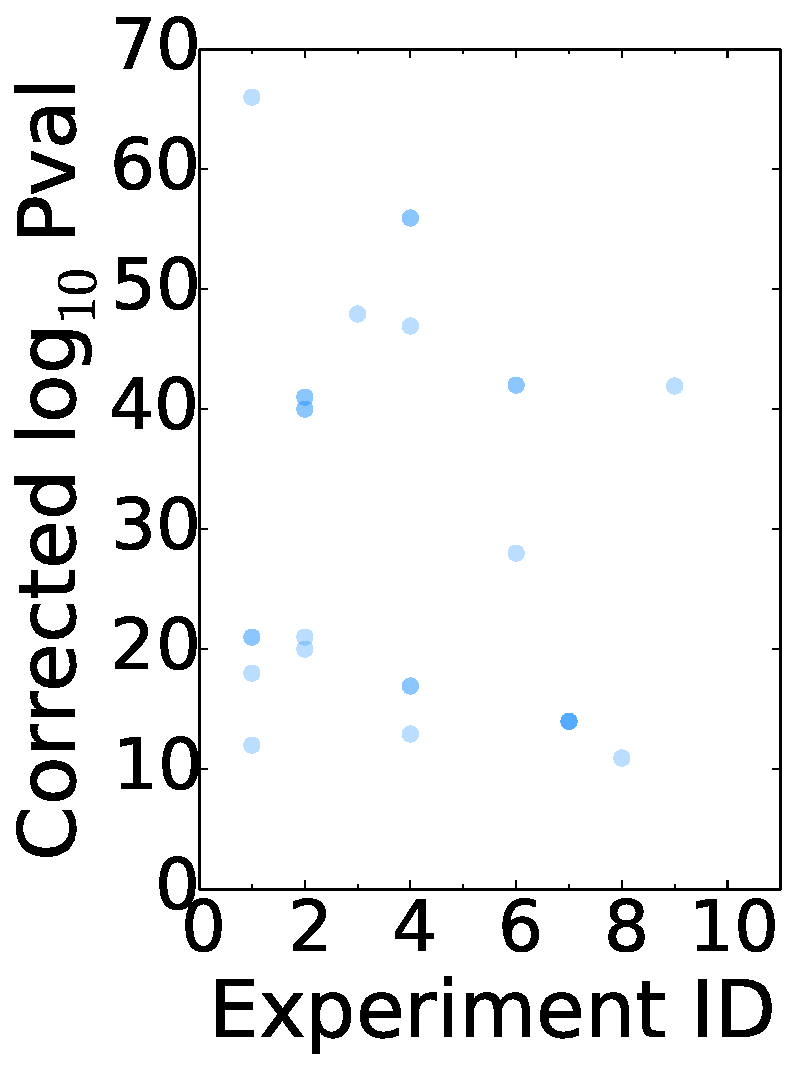
\includegraphics[width=.16\textwidth]{fig/msig_better_rank.pdf}}
% \subfigure[\lincs]{\label{fig:lincs_FP}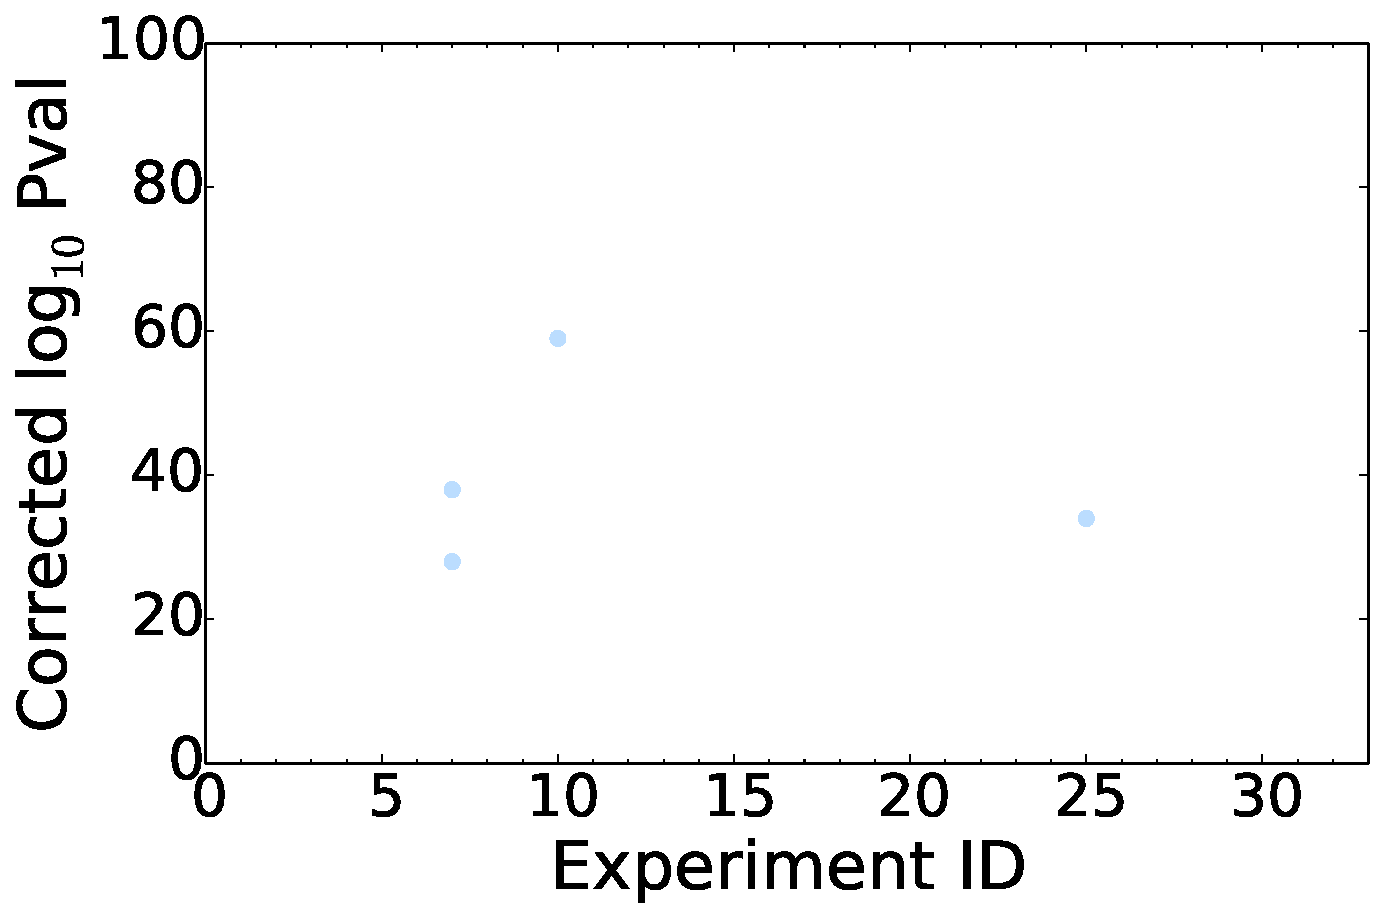
\includegraphics[width=.31\textwidth]{fig/lincs_better_rank.pdf}}
% \caption{Top-100 Feature Pairs' Corrected P-value Distribution}
% \label{fig:FP}
% \end{figure}

%\cb{I did not insert a substitute for this figure~\ref{fig:better_rank_20} (no longer referred to in the text and to be deleted). It may not be as necessary with some of the examples in the supplementary table.}

%\begin{figure}[h]
%\vspace{-5mm}
% \centering
% 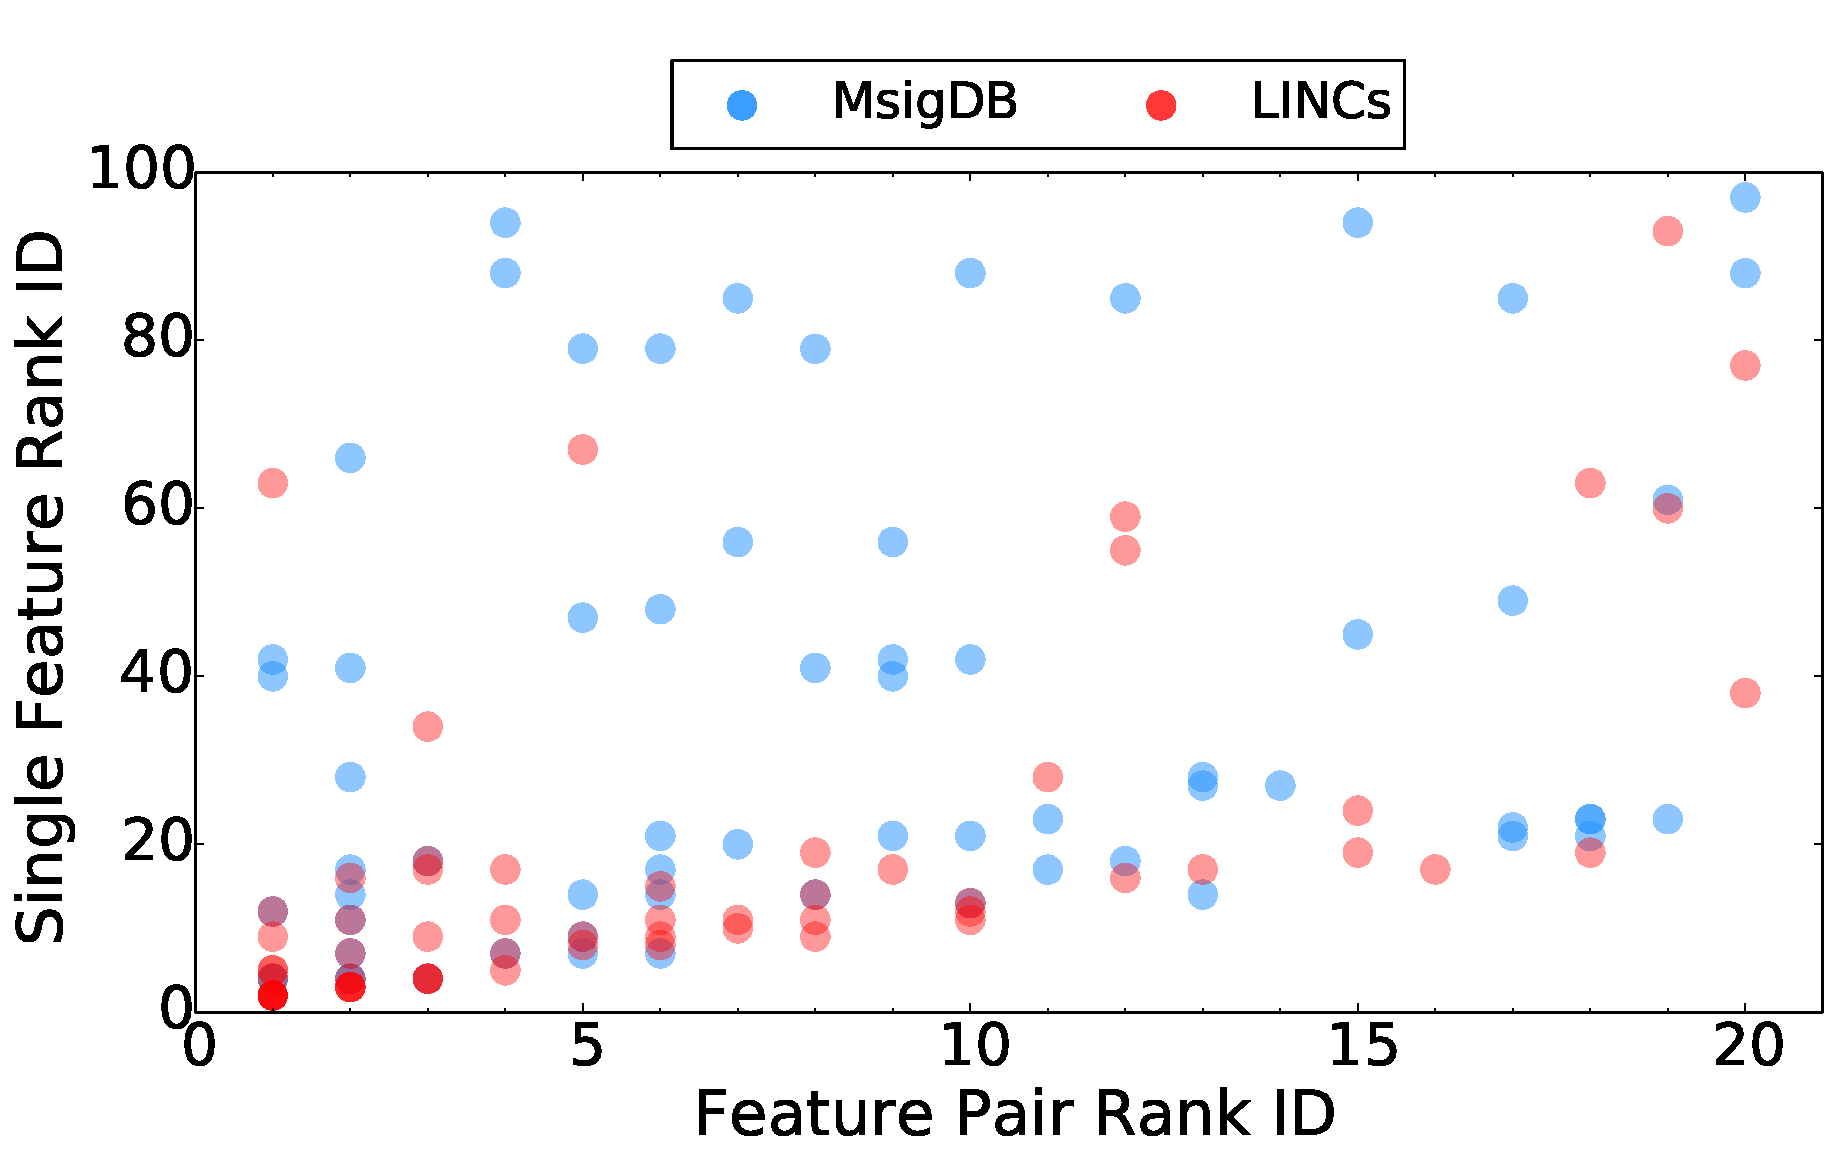
\includegraphics[width=0.8\linewidth]{fig/better_rank_20.pdf}
% \vspace{-5mm}
%\caption{Comparison of Feature Pair and Single Feature Rankings. The \toptwenty feature pairs from \msig (blue) and \lincs (red) datasets are depicted, with each circle representing a feature pair. The x-axis is the rank of the feature pair among all feature pair candidates, and y-axis is the better rank of its two individual single feature among all single features. The feature pair with the green circle is highlighted in the text. }
%\vspace{-5mm}
%\label{fig:better_rank_20}
%\end{figure}

%\sinha{why overlap the \msig and \lincs? suggests a simultaneous examination, which is not what we want here} \agp{yes}

%==================================================================
\subsection{Output Visualization}\label{ssec:viz}

\begin{figure}[h]
\centering %%% not \center
\vspace{-3mm}
\subfigure[\msig]{\label{fig:viz_msig}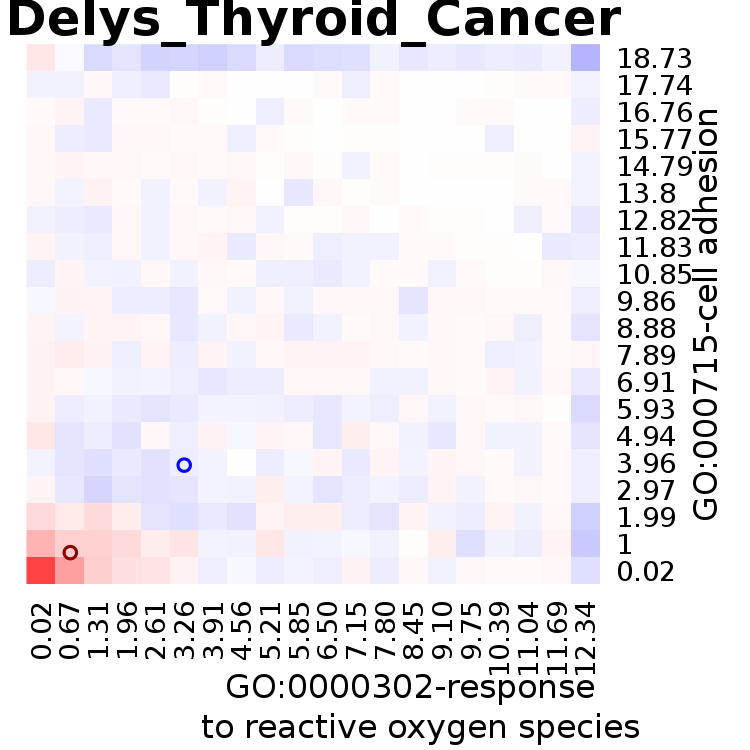
\includegraphics[width=.235\textwidth]{fig/ratioHist_msig_1.png}}
\subfigure[\lincs]{\label{fig:viz_lincs}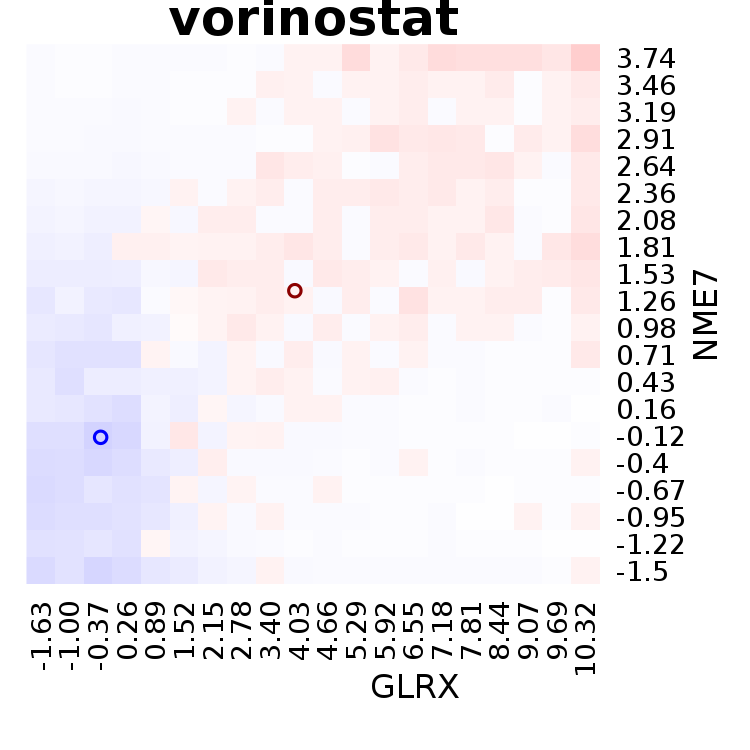
\includegraphics[width=.235\textwidth]{fig/ratioHist_newlincs_1.png}}
\vspace{-5mm}
\caption{Visualization Output of \genviz. Heatmap visualization with the pair of top features providing the x and y axes and the name of the run providing the plot title. The relative density of objects determines the color of the heatmap cells with blue indicating a greater proportion of positive objects and red indicating a greater proportion of negative objects. The class centroids are represented by blue and red circles, positive and negative classes respectively. The two examples shown are representatives from the (a) \msig and (b) \lincs datasets. }
\vspace{-5mm}
\label{fig:viz}
\end{figure}
\cb{silu, i think the colors in the figure are reversed from the legend. if so, can you change the figure? red for negative is more natural of bioinformatics}

As discussed in Section~\ref{sec:intro}, the output of \genviz is not simply a ranking of the top feature pairs with their separability scores, but also a visualization that helps users to interpret the separability of the object classes. In Figure~\ref{fig:viz}, we depict sample output visualizations from the \msig and \lincs runs. For \msig, we select the feature pair with the highest improved p-value, i.e., $improv\_quot$, using the \sampOpt algorithm. For our \lincs representative, we visualize the gene feature pair (GLRX, NME7) for the drug vorinostat as described in the previous section. We use a heatmap to illustrate the distribution of positive objects (in blue) and negative objects (in red) under the selected feature pair $(f_i,f_j)$, where $f_i$ is x-axis, $f_j$ is y-axis. The color represents the difference between the weighted number of positive objects and negative objects. If the number of positive objects is larger than negative objects in the cell, the cell is colored as blue, otherwise, it is red. For the ease of interpretation, we also add the centroids of positive and negative objects using blue circle and red circle respectively. For the \msig example (Figure~\ref{fig:viz}(a)) \cb{relates (DELYS\_THYROID\_CANCER\_DN, response to reactive oxygen species, cell adhesion) which consistent with role of cell adhesion in cancer prognosis}, we observe that the feature values for negative objects is clustered around zero, while positive objects have larger values overall, indicating stronger network relationships to the feature Gene Ontology terms. For the \lincs example (Figure~\ref{fig:viz}(b)), positive objects mostly have elevated expression for the selected gene significantly different from the negative objects with zero-mean Gaussian distribution. The direction of this differential gene expression for both genes is consistent with literature for vorinostat experiments \needcite{CTD pubmeds: 22083351, 27188386}. These above two examples illustrate how visualization of significant feature pairs can be a useful way to explain the separability of object sets and understand the data.



\section{Discussion}\label{sec:disc}
\cb{SS would like us to figure out how to make a simple interface for this. so we need a design of configure page, design of results page, and examples how to call backend code}

\cb{for the discussion: non-linear features?}

\cb{Low priority, but I am interested in knowing for all the feature pairs we return that are better/new. what type of relationship between the pair are we finding. maybe captured by the slope of the perp bisector?}

\cb{again low priority, but how robust are these results. If you run a sampling method twice, do you get the same feature pairs. if you change the positive set slightly, are your results comparable?}


\appendix
\section{Appendix}\label{sec:supplement}

\begin{table*}[t]
\centering
\small
\begin{tabular}{|c|c|c|c|c|c|c|c|c|c|c|c|}
 \hline
 & & \multirow{ 2}{*}{\baseline} & \multirow{ 2}{*}{\earlyOrder} & \multicolumn{2}{c|}{\samp}
& \multicolumn{2}{c|}{\sampOpt} & \multicolumn{2}{c|}{\horiz} & \multicolumn{2}{c|}{\vertic} \\
  \cline{5-12}
& & & & Phase 1 & Phase 2
& Phase 1 & Phase 2 & Phase 1 & Phase 2 & Phase 1 & Phase 2 \\
  \hline
\multirow{ 2}{*}{\msig} & FPs Checked & $2\times 10^8$ & $2\times 10^8$ & $2\times 10^8$ & $4.1\times 10^6$ & $1.9 \times 10^8$ & $2.3\times 10^6$ & $10^7$ & $1.2\times 10^6$ & $10^7$ & $5.5\times 10^5$ \\
\cline{2-12}
 & Objects Checked & 22209 & 5427 & 694 & 22209 & 694 & 22209 & 694 & 22209 & 694 & 22209 \\
  \hline
\multirow{ 2}{*}{\lincs} & FPs Checked & $2.5\times 10^8$ & $2.5\times 10^8$ & $2.5\times 10^8$ & $3.3\times 10^5$ & $2.5\times 10^8$ & $9.1\times 10^4$ & $10^7$ & $8.6\times 10^4$ & $10^7$ & $5.0\times 10^4$\\
\cline{2-12}
 & Objects Checked & 98061 & 15631 & 564 & 98061 & 564 & 98061 & 564 & 98061 & 564 & 98061 \\
  \hline
  \end{tabular}
\caption{Supplement Table for Running Time Comparison in Figure~\ref{fig:time}. FPs represents feature pairs.}
\label{tbl:supplement}
\end{table*}


\eat{

xxx[y]

[y]}





{\scriptsize
\bibliographystyle{abbrv}
\bibliography{ref}
}
\end{document}
